\documentclass[12pt]{article}
\usepackage{amssymb}
\usepackage{amsmath}
\usepackage{mathtools}
\usepackage[utf8]{inputenc}
\usepackage{hyperref}
\usepackage{comment}
\usepackage{polski}
\usepackage{mathrsfs}
\usepackage{geometry}
\usepackage{amsthm}
\usepackage{csquotes}
\usepackage{float}
\geometry{a4paper, portrait, margin=1in}

\usepackage[breaklinks=true]{hyperref}

\setlength\parindent{0pt}

\DeclarePairedDelimiter\abs{\lvert}{\rvert}%
\DeclarePairedDelimiter\norm{\lVert}{\rVert}%

% Swap the definition of \abs* and \norm*, so that \abs
% and \norm resizes the size of the brackets, and the 
% starred version does not.
\makeatletter
\let\oldabs\abs
\def\abs{\@ifstar{\oldabs}{\oldabs*}}
%
\let\oldnorm\norm
\def\norm{\@ifstar{\oldnorm}{\oldnorm*}}
\makeatother

\newcommand{\Cov}{\mathrm{Cov}}
\newcommand{\corr}{\mathrm{corr}}
\newcommand{\pH}{\mathscr{H}}
\newcommand{\bH}{\mathscr{B}(\mathscr{H})}
\newcommand{\gH}{\mathscr{G}(\mathscr{H})}
\newcommand{\complex}{\mathbb{C}}
\newcommand{\real}{\mathbb{R}}
\newcommand*\conj[1]{\overline{#1}}
\newcommand*\dotprod[2]{\langle #1 , #2 \rangle}
\newtheorem{theorem}{Twierdzenie}[section]
\newtheorem{corollary}{Wniosek}[theorem]
\newtheorem{lemma}[theorem]{Lemat}
\newtheorem{fact}[theorem]{Fakt}
\newtheorem{definition}[theorem]{Def.}
\newtheorem{example}[theorem]{Pd.}
\newcommand{\pder}[2][]{\frac{\partial#1}{\partial#2}}
% Command for partial derivatives. The first argument denotes the function and the second argument denotes the variable with respect to which the derivative is taken. The optional argument denotes the order of differentiation. The style (text style/display style) is determined automatically
\providecommand{\pd}[3][]{\ensuremath{
\ifinner
\tfrac{\partial{^{#1}}#2}{\partial{#3^{#1}}}
\else
\dfrac{\partial{^{#1}}#2}{\partial{#3^{#1}}}
\fi
}}

\title{Projekt II - finite difference and uncertain parameters.}
\author{Wojciech Fica \footnote{\href{mailto:wojtekfica@gmail.com}{wojtekfica@gmail.com}}, Krzysztof Krawiec \footnote{\href{mailto:krzkra56@gmail.com}{krzkra56@gmail.com}}, Wojciech Prokopowicz \footnote{\href{mailto:wojtpro@interia.pl}{wojtpro@interia.pl}}}
\date{\today}

\begin{document}

\maketitle
%\tableofcontents
%\pagebreak

\section{Wstęp}
W projekcie zakładamy, że jest dziś 1 stycznia 2020 roku. Celem projektu jest zaimplementowanie metody explicite finite difference i przy jej użyciu przeprowadzenie analizy opcji:
\begin{enumerate}
    \item opcje europejskie call knock-and-out,
    \item opcje europejskie put knock-and-out,
    \item opcje amerykańskie call knock-and-out,
    \item opcje amerykańskie put knock-and-out.
\end{enumerate}
W projekcie zakładamy niepewną zmienność z przedziału [15\%, 25\%], i zapadalność rozważanych opcji na dzień 30 września 2020. 

\textbf{Uwaga notacyjna:} W związku z powyższym, na wykresach $t=0$ symbolizuje 1 stycznia 2020, $t=1$  - 31 grudnia 2020, a $t=0.7$  - 30 września 2020.

\section{Wpływ zmiany parametrów na cenę opcji europejskich.}
Pokażemy teraz jak wyglądają ceny opcji gdy modyfikujemy różne parametry. Zaczniemy od najprostszego modelu i będziemy stopniowo zwiększać liczbę parametrów.  

\subsection{Opcje europejskie, stała zmienność.}

Wykresy \ref{fig:ec_2150_fixed_vol} i \ref{fig:ep_2150_fixed_vol} przedstawiają cenę opcji EC@2150  i EP@2150, odpowiednio, gdy założymy stałą zmienność $\sigma = 20\%.$ Otrzymane ceny w chwili $t=0$  (1 stycznia 2020) zgadzają się ze wzorami analitycznymi wyprowadzonymi z formuły B-S.
\begin{figure}[H]
    \centering
    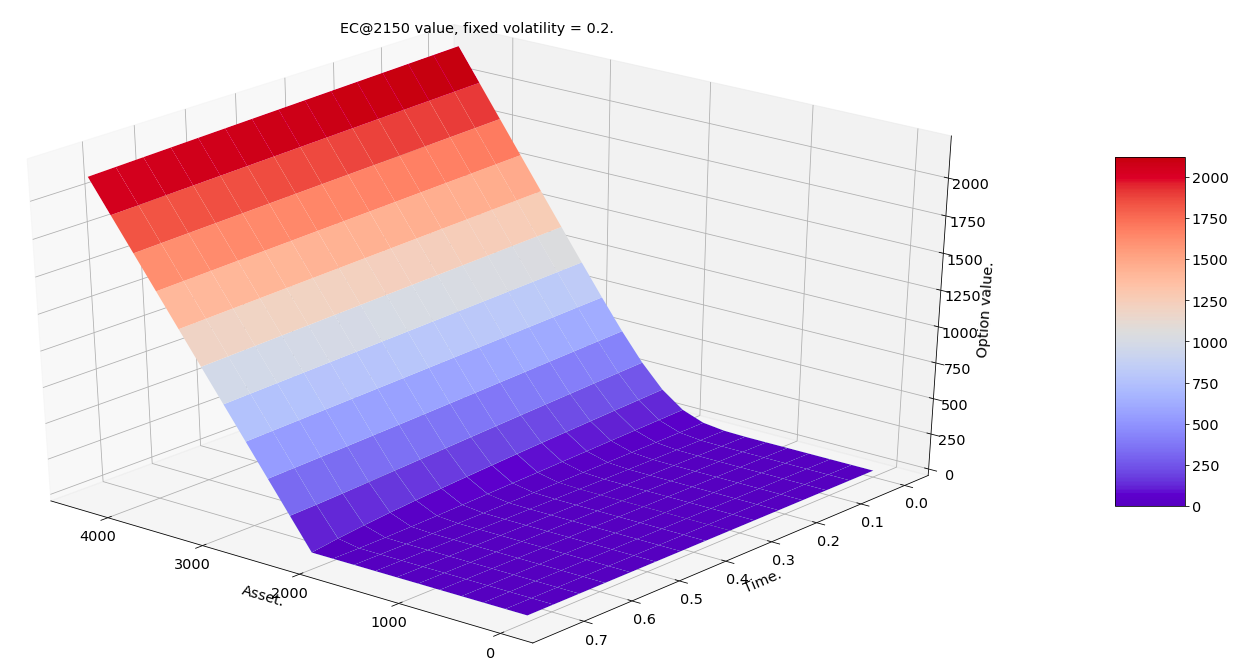
\includegraphics[width=\textwidth,height=\textheight,keepaspectratio]{ec_2150_fixed_vol.png.png}
    \caption{EC@2150, $\sigma = 20\%.$}
    \label{fig:ec_2150_fixed_vol}
\end{figure}

\begin{figure}[H]
    \centering
    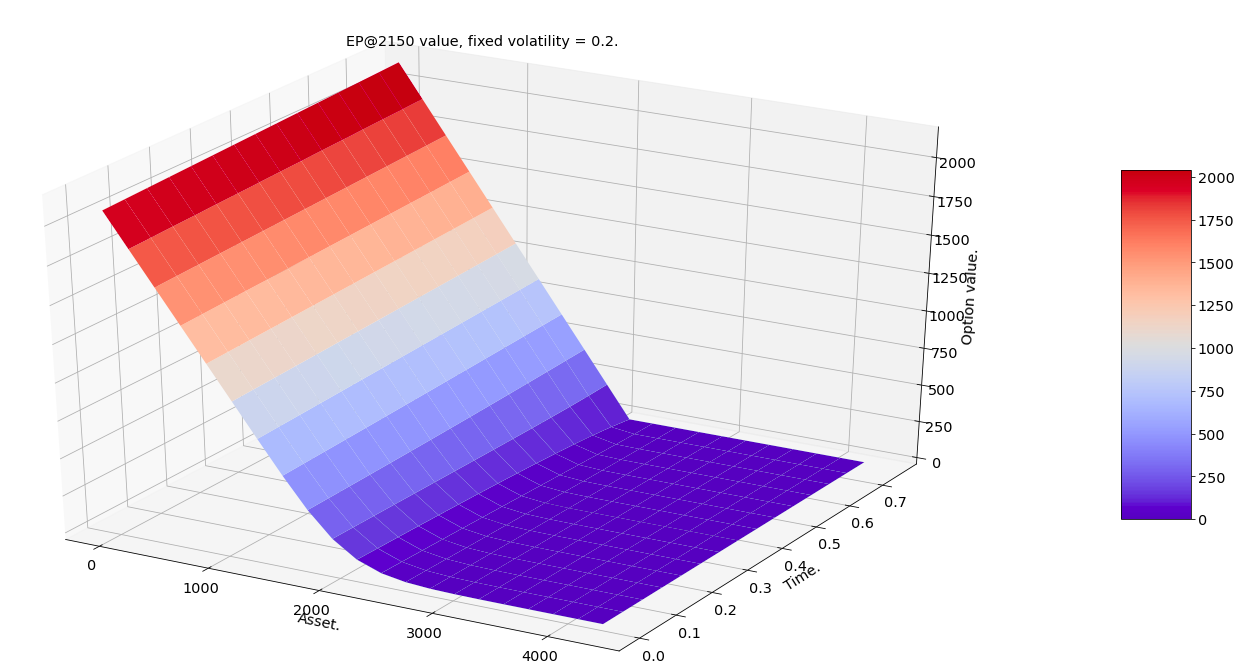
\includegraphics[width=\textwidth,height=\textheight,keepaspectratio]{ep_2150_fixed_vol.png}
    \caption{EP@2150, $\sigma = 20\%.$}
    \label{fig:ep_2150_fixed_vol}
\end{figure}

\newpage

\subsection{Opcje europejskie, nieznana zmienność.}

Wykresy \ref{fig:ec_2150_uncer_vol} i \ref{fig:ep_2150_uncer_vol} przedstawiają cenę opcji EC@2150  i EP@2150, odpowiednio, gdy założymy stałą nieznaną zmienność $\sigma \in [15\%, 25\%].$ Aby zobaczyć różnicę z poprzednią sytuacją, gdy mieliśmy znaną stałą zmienność warto spojrzeć na wykres \ref{fig:value_ec_ep_uncert_vol_t_0}. Przedstawia on ceny opcji w 3 sytuacjach:
\begin{enumerate}
    \item $\sigma = 15\%.$
    \item $\sigma = 25\%.$
    \item $\sigma \in [15\%, 25\%].$
\end{enumerate}
Widzimy, że zarówno dla opcji Call jak i Put wartość instrumentu przy nieznanej zmienności z przedziału [15\%, 25\%] pokrywa się z wartością instrumentu gdybyśmy założyli zmienność stałą równą  25\%. Zgadza się to z wyprowadzonym na wykładzie modelem gdzie zakładamy 'pesymistyczny scenariusz'. Poniżej wyjaśnienie.   Jesteśmy w sytuacji, gdy sprzedajemy opcję i ją zabezpieczamy. Nasz portfel to 
$$
    \Pi = -V + \Delta S.
$$
Korzystając ze wzoru Ito, piszemy:
$$
- d\Pi = (\pd{V}{t} + \frac{1}{2}\sigma^2S^2 \pd[2]{V}{S})dt + (\pd{V}{S} -\Delta) dS
$$
Eliminujemy losowość poprzez delta-hedging. 
$$
\Delta = \pd{V}{S}
$$
W każdym momencie zakładamy, że wartość naszego portfela rośnie o minimalną możliwą kwotę. Wtedy zwrot z takiego pesymistycznego portfela jest równy zwrotowi z inwestycji wolnej od ryzyka.
$$
\min_{\sigma_{\min} < \sigma < \sigma_{\max} } (d \Pi) = r \Pi dt.
$$
Stąd
$$
\min_{\sigma^- < \sigma < \sigma^+ } -(\pd{V}{t} + \frac{1}{2}\sigma^2S^2 \pd[2]{V}{S})dt  = r (-V + \pd{V}{S} S) dt.
$$
Czyli 
$$
 -(\pd{V}{t} + \frac{1}{2}\sigma^2(\Gamma)S^2 \pd[2]{V}{S}) =r (-V + \pd{V}{S} S),  
$$
gdzie 
\begin{equation*}
    \sigma(\Gamma) = 
    \begin{cases} 
        \sigma_{\max}, & \text{jeśli}\ \Gamma \geq 0 \\
        \sigma_{\min}, & \text{jeśli}\ \Gamma < 0 \\
    \end{cases}
\end{equation*}
    
W tym modelu zmienność zależy tylko od znaku gammy. A gamma dla opcji call i put jest taka sama i \textbf{stale dodatnia}.
$$
\Gamma_{Call} = \Gamma_{Put} = \frac{N'(d_1)}{\sigma S \sqrt{T-t}} \geq 0.
$$

\begin{figure}[H]
    \centering
    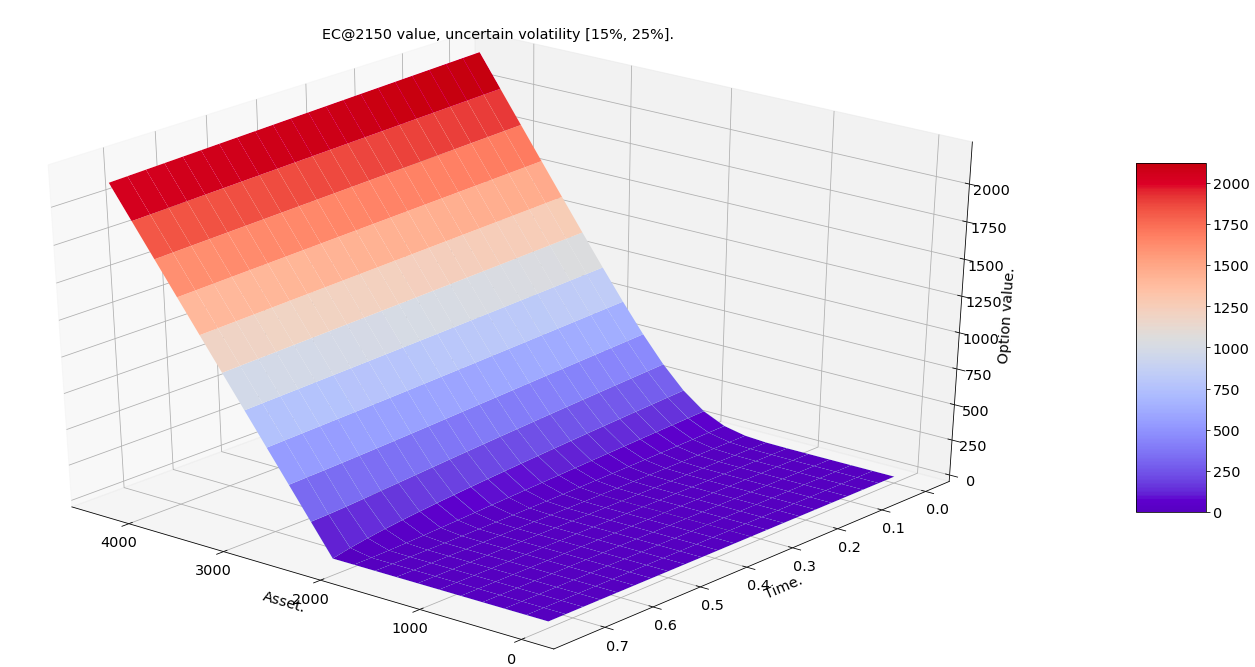
\includegraphics[width=\textwidth,height=\textheight,keepaspectratio]{EC_2150_uncert_vol.png}
    \caption{EC@2150, $\sigma \in [15\%, 25\%].$}
    \label{fig:ec_2150_uncer_vol}
\end{figure}

\begin{figure}[H]
    \centering
    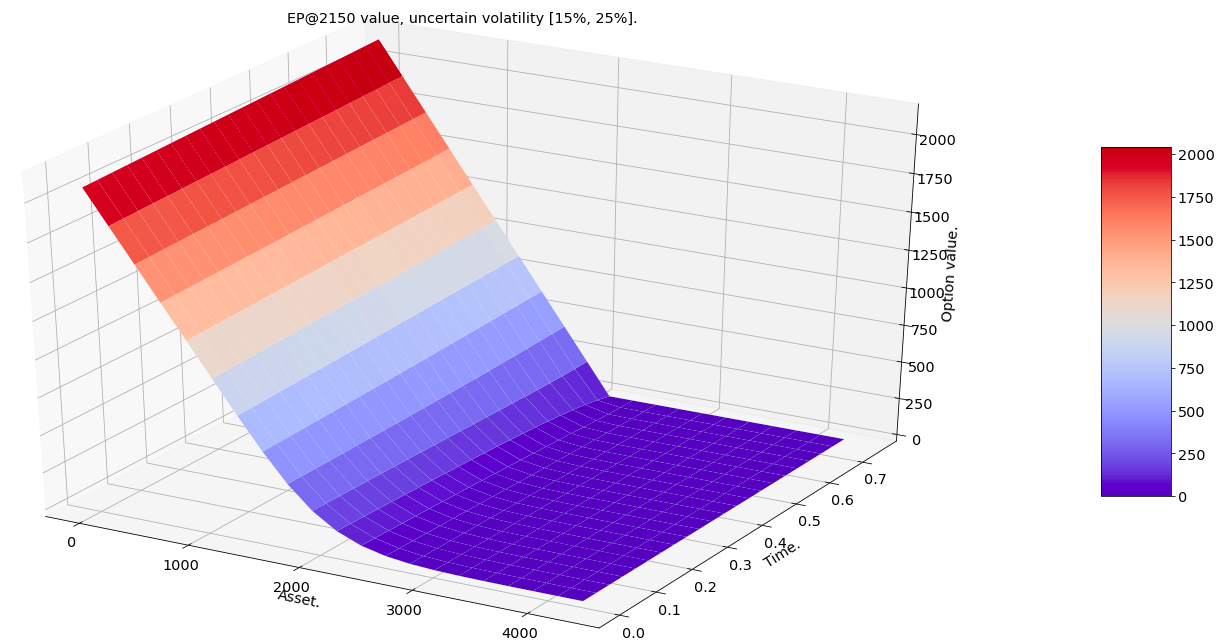
\includegraphics[width=\textwidth,height=\textheight,keepaspectratio]{ep_2150_uncert_vol.png}
    \caption{EP@2150, $\sigma \in [15\%, 25\%].$}
    \label{fig:ep_2150_uncer_vol}
\end{figure}

\begin{figure}[H]
    \centering
    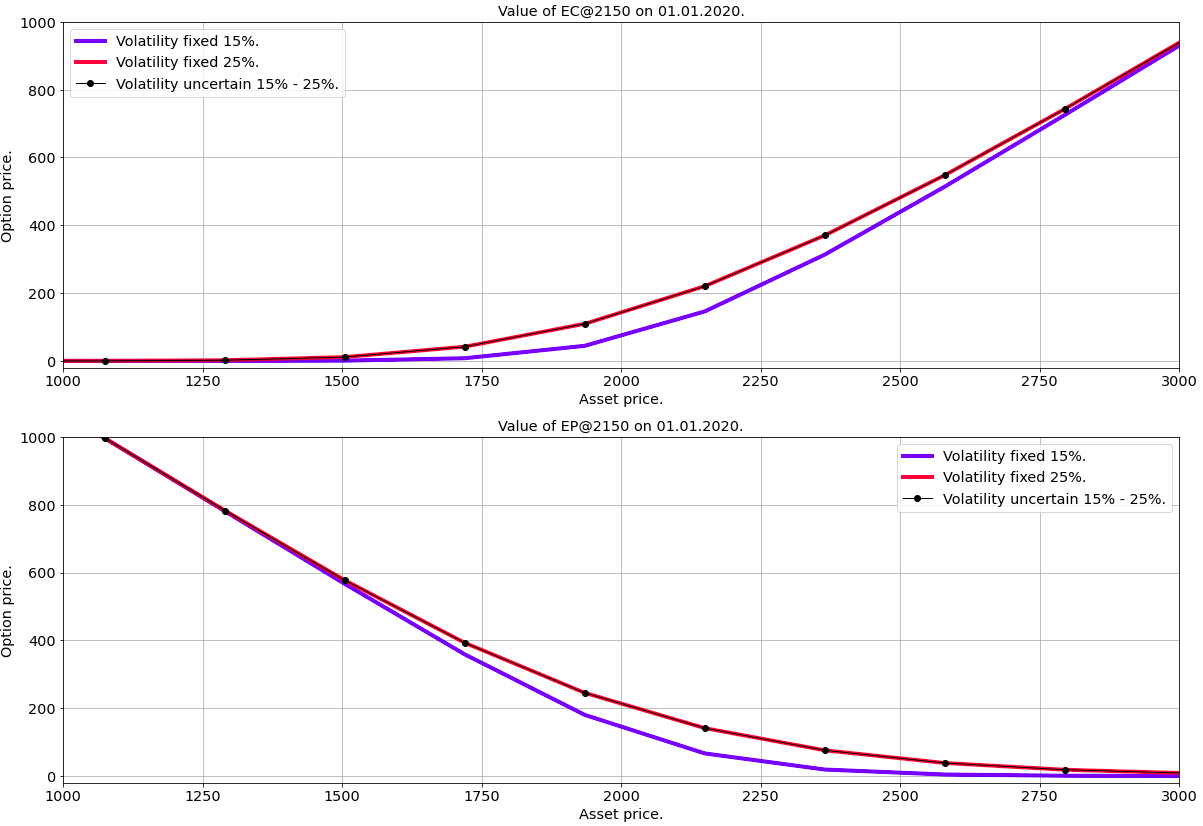
\includegraphics[width=\textwidth,height=\textheight,keepaspectratio]{value_ec_ep_uncert_vol_t_0.png}
    \caption{Wartość EC@2150 i EP@2150 w dniu 1 styczna 2020, przy $\sigma \in [15\%, 25\%].$}
    \label{fig:value_ec_ep_uncert_vol_t_0}
\end{figure}


\subsection{Opcje europejskie, barierowe, nieznana zmienność.}
Przedstawimy teraz wyniki dla europejskiej opcji call z ceną wykonania 2150 i barierą knock-and-out 2400 przy nieznanej zmienności z przedziału [15\%, 25\%]. 

Wykres  \ref{fig:ec_2150_b_2400_uv} przedstawia cenę opcji EC@2150 knock-and-out 2400, $\sigma \in [15\%, 25\%].$ Widzimy, że znacząco różni się on od poprzednich wykresów cen opcji call. Aby dokładniej zobrazować co się dzieję warto spojrzeć na kolejny wykres (\ref{fig:ec_2150_b_2400_different_dates}), który przedstawia ceny tej opcji w kilku różnych dniach. Widzimy, że im bliżej momentu wykonania, 
\begin{enumerate}
    \item tym bardziej wykres zbliża się do standardowego payoffu opcji call dla wartości z dala od bariery,
    \item tym bardziej zaostrza się spadek dla wartości przy barierze.
\end{enumerate} 
Takie zachowanie zgadza się z intuicjami ekonomicznymi. 

\begin{figure}[H]
    \centering
    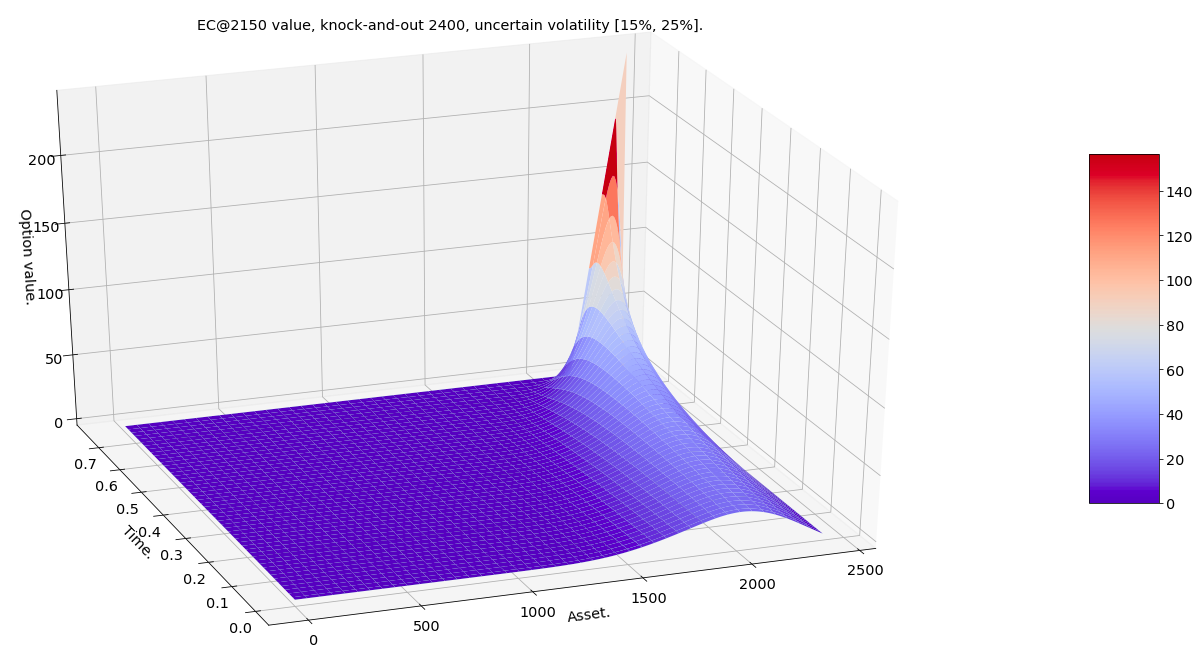
\includegraphics[width=\textwidth,height=\textheight,keepaspectratio]{ec_2150_b_2400_uv.png}
    \caption{EC@2150 knock-and-out 2400, $\sigma \in [15\%, 25\%].$}
    \label{fig:ec_2150_b_2400_uv}
\end{figure}

\begin{figure}[H]
    \centering
    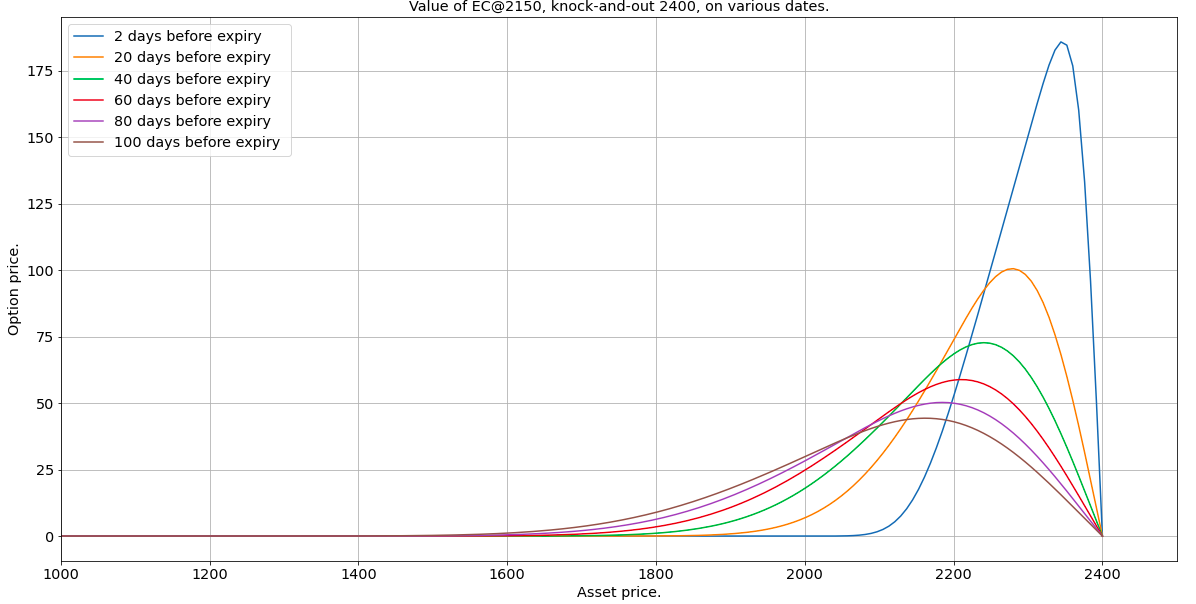
\includegraphics[width=\textwidth,height=\textheight,keepaspectratio]{ec_2150_b_2400_various_dates.png}
    \caption{EC@2150 knock-and-out 2400, $\sigma \in [15\%, 25\%].$}
    \label{fig:ec_2150_b_2400_different_dates}
\end{figure}

\subsubsection{Zmienność pewna vs niepewna.}
Wykres \ref{fig:ec_2150_b_2400_90_days_uncertain_vs_fixed} pokazuje wartość opcji EC@2150 knock-and-out 2400 na 90 dni przed momentem wykonania w sytuacjach gdy mamy zmienność ustaloną oraz gdy jest ona niepewna. Widzimy, że w tym wypadku wartość opcji z $\sigma \in [15\%, 25\%]$ nie pokrywa się ani z wartością dla $\sigma=15\%$, ani z wartością dla $\sigma=25\%$. Zgadza się to z wyprowadzonym na wykładzie modelem. 

\begin{figure}[H]
    \centering
    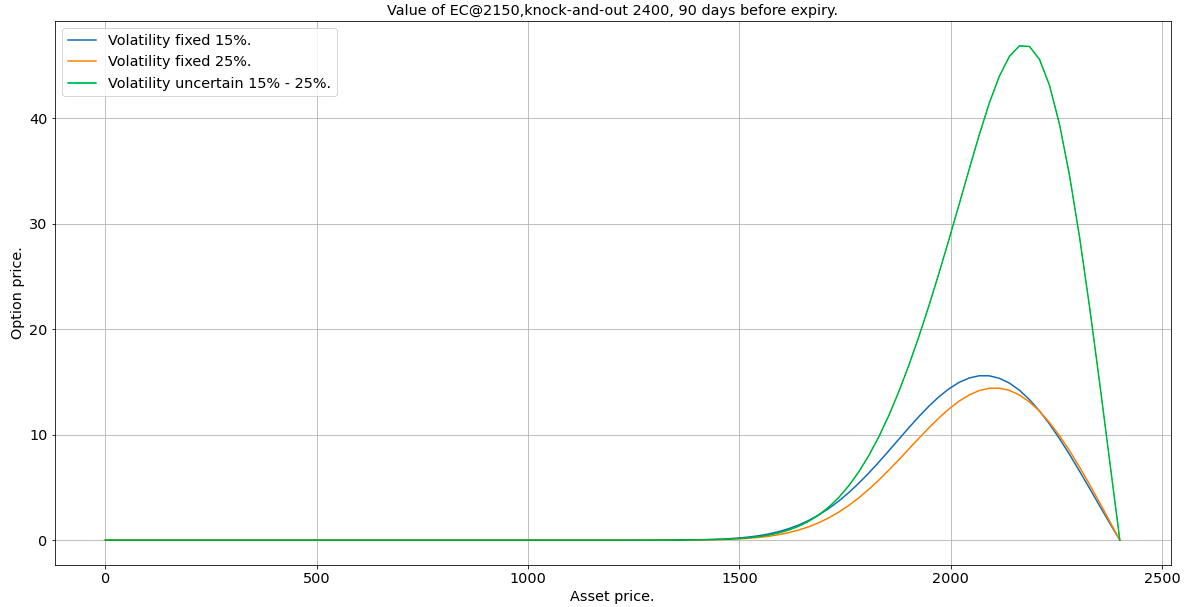
\includegraphics[width=\textwidth,height=\textheight,keepaspectratio]{ec_2150_b_2400_90_days_uncertain_vs_fixed.png}
    \caption{Wartość EC@2150, knock-and-out 2400, 90 dni przed wygaśnięciem, różne zmienności.}
    \label{fig:ec_2150_b_2400_90_days_uncertain_vs_fixed}
\end{figure}

\subsubsection{Różne przedziały zmienności.}
Porównamy teraz jak zmiana przedziału możliwych wartości zmienności wpływa na cenę opcji. Wykres \ref{fig:ec_2150_b_2400_uv_10_30} przedstawia cenę opcji EC@2150 knock-and-out 2400, $\sigma \in [10\%, 30\%].$ 
\begin{figure}[H]
    \centering
    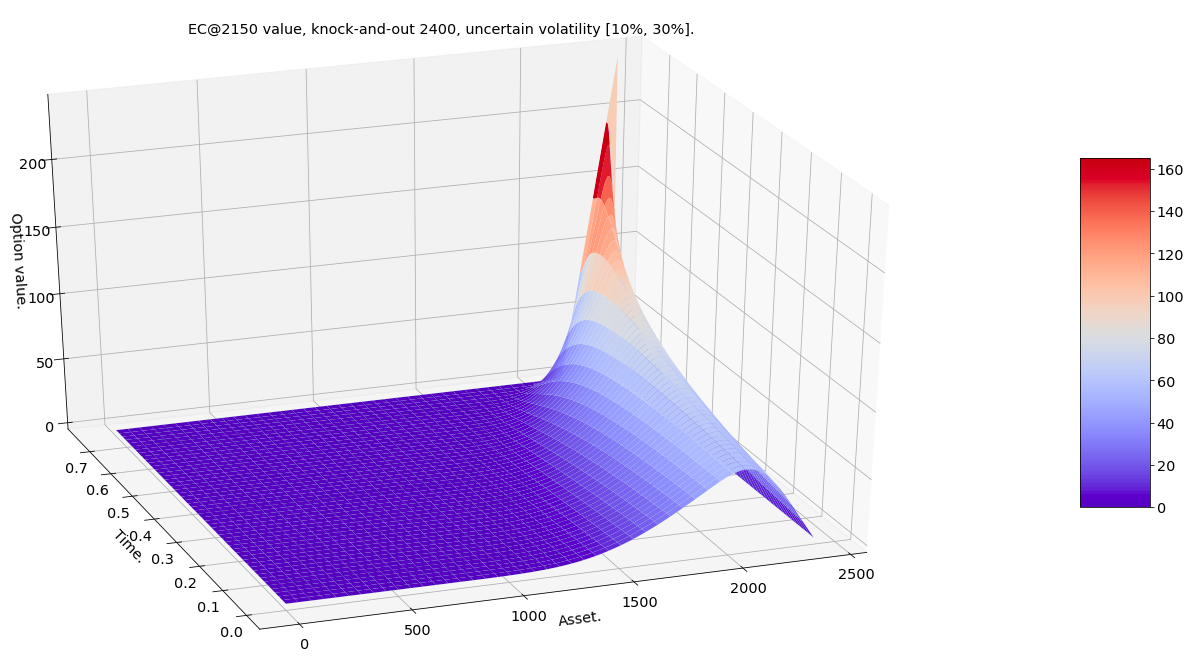
\includegraphics[width=\textwidth,height=\textheight,keepaspectratio]{ec_2150_b_2400_uv_10_30.png}
    \caption{EC@2150 knock-and-out 2400, $\sigma \in [10\%, 30\%].$}
    \label{fig:ec_2150_b_2400_uv_10_30}
\end{figure}

Warto porównać go z wykresem \ref{fig:ec_2150_b_2400_uv}, w którym wszystkie parametry były takie same, ale  zmienność była z innego przedziału: $\sigma \in [15\%, 25\%].$ Aby lepiej to zobrazować zobaczmy jak zmiana przedziału niepewności zmienności wpływa na cenę opcji w dniu 1 stycznia 2020 - wykres \ref{fig:ec_2150_b_2400_var_vol}. Widzimy, że im szerszy przedział zmienności, tym więcej opcja jest warta. 
\begin{figure}[H]
    \centering
    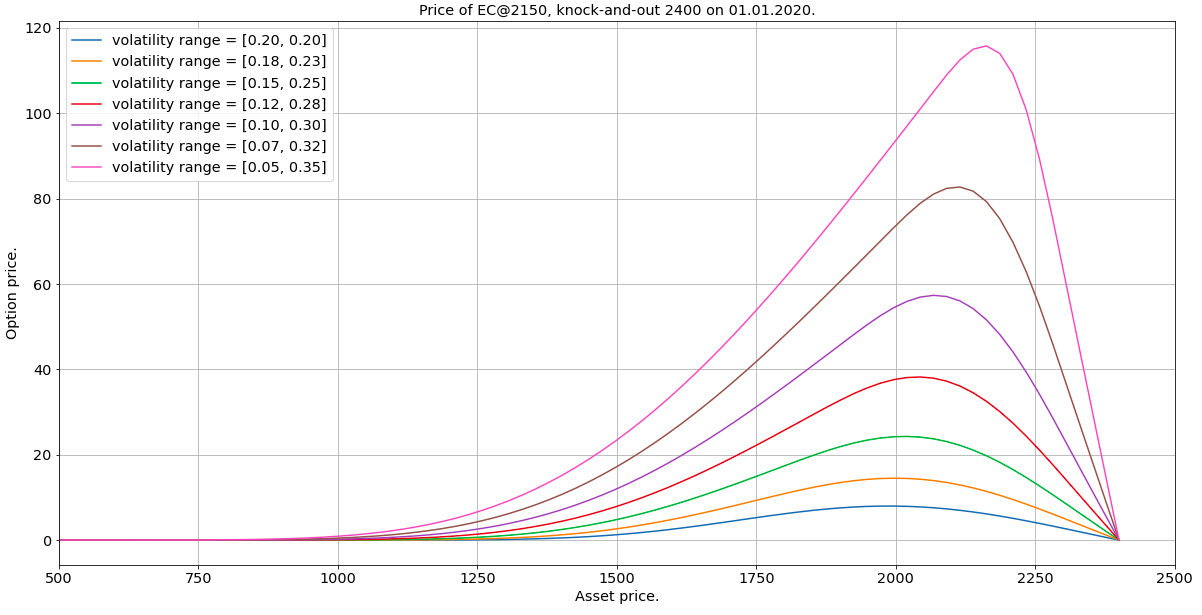
\includegraphics[width=\textwidth,height=\textheight,keepaspectratio]{ec_2150_b_2400_var_vol.png}
    \caption{Wartość EC@2150, knock-and-out 2400, 01.01.2020r., różne zakresy niepewnej zmienności.}
    \label{fig:ec_2150_b_2400_var_vol}
\end{figure}

\subsubsection{Opcje put.}

Aby raport był pełny przedstawiamy jeszcze wykres ceny opcji europejskiej put z ceną wykonania 2150 i barierą knock-and-out 1900 - wykres \ref{fig:ep_2150_1900_uv}.

\begin{figure}[H]
    \centering
    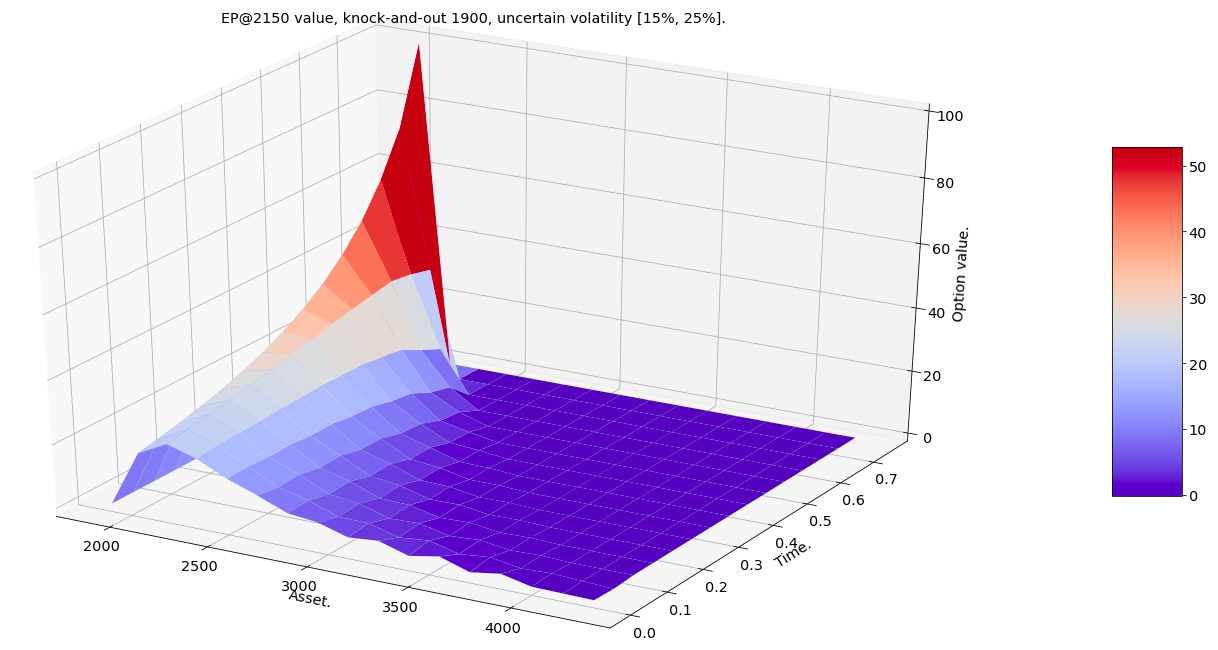
\includegraphics[width=\textwidth,height=\textheight,keepaspectratio]{ep_2150_1900_uv.png}
    \caption{Wartość EP@2150, knock-and-out 1900, $\sigma \in [15\%, 25\%].$}
    \label{fig:ep_2150_1900_uv}
\end{figure}

\section{Wpływ zmiany parametrów na cenę opcji amerykańskich.}
\subsection{Opcje amerykańskie call.}

W tym rozdziale wyjaśnimy wpływ parametrów na wartość opcji amerykańskich. Będziemy analizować opcje barierowe typu knock-and-out. 

Wykres \ref{fig:ac_2150_2400_uv} przedstawia cenę AC@2150 typu knock-and-out 2400, gdzie $\sigma \in [15\%, 25\%].$ Więcej szczegółów można zobaczyć na wykresie \ref{fig:ac_2150_2400_diff_dates}, który przedstawia ceny tej opcji w kilku różnych momentach czasu. Widzimy znaczną zmianę pomiędzy wyceną opcji amerykańskich a europejskich. Przy zbliżaniu się ceny aktywa podstawowego do bariery, ceny opcji europejskich wyraźnie traciły na wartości. Intuicyjnie można to wytłumaczyć tak, że inwestorzy obawiają się, że cena urośnie / spadnie do bariery i opcja stanie się bezwartościowa. Przy opcjach amerykańskich sytuacja wygląda całkiem inaczej. Gdy cena aktywa zbliża się do bariery, to cena opcji się nie zmniejsza, przeciwnie, zwiększa się. Dzieje się tak dlatego, ponieważ opcję amerykańską można zawsze wykonać, więc można taką opcję 'trzymać' i wykonać ją na sekundę przed uderzeniem w barierę. Dodatkowo, na wykresie \ref{fig:ac_2150_2400_diff_dates} widać, że cena opcji amerykańskiej barierowej jest zawsze większa równa od payoffu. Opcje europejskie barierowe nie miały tej własności. 
\begin{figure}[H]
    \centering
    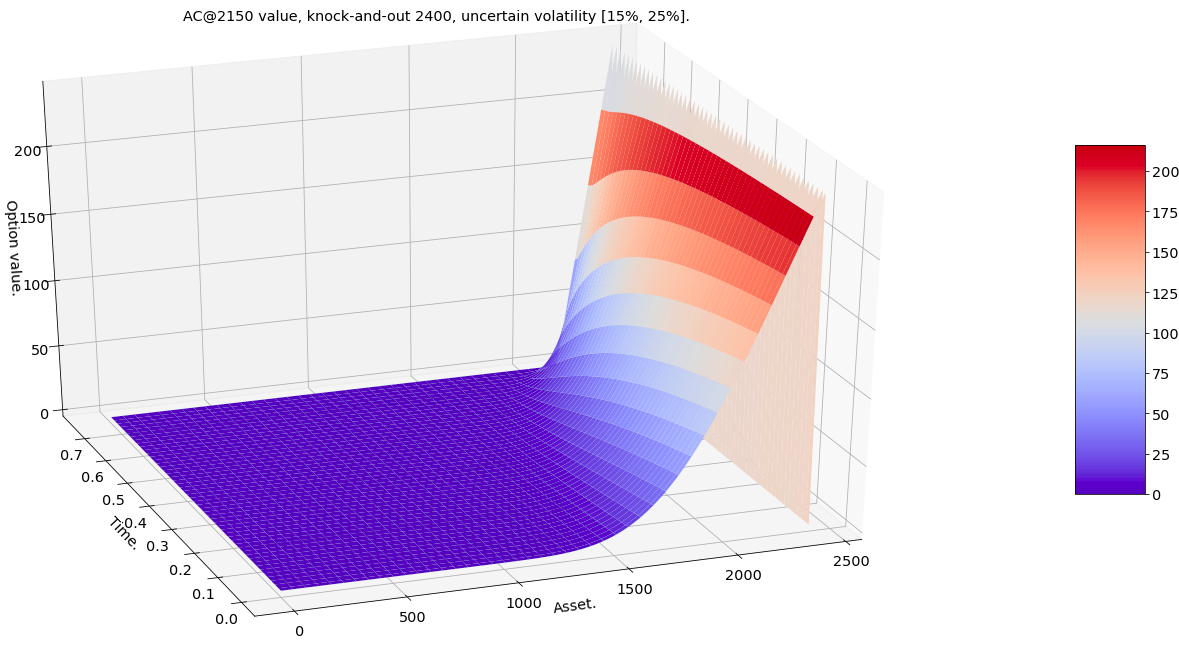
\includegraphics[width=\textwidth,height=\textheight,keepaspectratio]{ac_2150_2400_uv.png}
    \caption{Wartość AC@2150, knock-and-out 2400, $\sigma \in [15\%, 25\%].$}
    \label{fig:ac_2150_2400_uv}
\end{figure}

\begin{figure}[H]
    \centering
    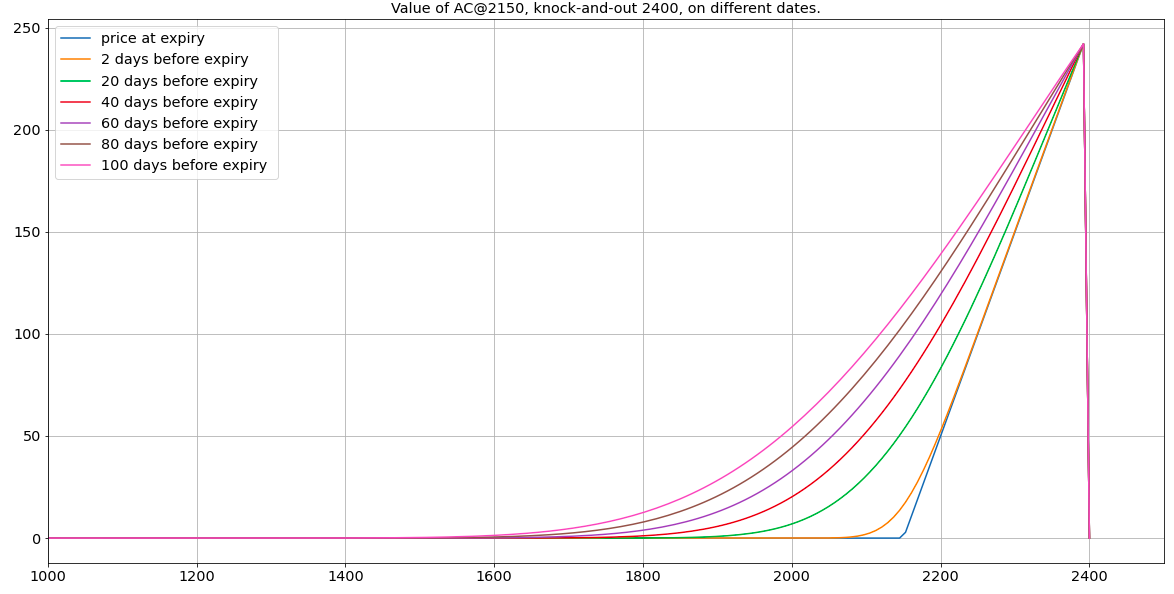
\includegraphics[width=\textwidth,height=\textheight,keepaspectratio]{ac_2150_2400_diff_dates.png}
    \caption{Wartość AC@2150, knock-and-out 2400, $\sigma \in [15\%, 25\%],$ różne daty.}
    \label{fig:ac_2150_2400_diff_dates}
\end{figure}

\subsubsection{Wpływ przedziału zmienności na opcje europejskie.}

Zobaczmy teraz jak zmiana przedziału niepewnej zmienności wpływa na wycenę opcji amerykańskich w dniu 1 stycznia 2020 - wykres \ref{fig:ac_2150_2400_diff_vol_range}. Tak jak przy opcjach europejskich im większa zmienność, tym więcej warta jest opcja. Intuicyjnie można wysnuć hipotezę, że gdy mamy większy możliwy zakres zmienności, to musimy zabezpieczyć się na więcej możliwych scenariuszy. Chcąc to zweryfikować, popatrzymy na wykres \ref{fig:ac_2150_2400_diff_vol_ex}. Przedstawia on wycenę opcji amerykańskich w dniu 1 stycznia 2020 dla różnych przedziałów zmienności, ale tym razem te przedziały są rozłączne. Widzimy, że im większa zmienność, tym więcej warta jest opcja. Można to próbować wyjaśnić mówiąc, że 
\begin{enumerate}
    \item jeśli zmienność jest mała, rzędu [5\%, 10\%], to cena aktywa podstawowego nie zmieni się zbytnio przez 9 miesięcy, zatem cena opcji w dniu 1 styczna 2020 powinna przypominać payoff z dnia 30 września 2020.  
    \item przy zmienności rzędu [5\%, 10\%] prawdopodobieństwo, że cena aktywa podstawowego urośnie lub zmaleje o 100 punktów jest mała. 
    \item gdy zmienność jest większa, rzędu [25\%, 30\%], to cena aktywa podstawowego bardziej się zmienia.  Wtedy jest większa szansa i na to, że cena aktywa podstawowego urośnie o 100 punktów, i na to że zmaleje o 100 punktów w porównaniu do poprzedniego punktu.  
    \item w związku z tym, że przy $\sigma \in [25\%, 30\%]$ jest większa szansa na to, że cena urośnie, niż przy $\sigma \in [5\%, 10\%],$ to cena opcji przy $\sigma \in [25\%, 30\%]$ powinna być wyższa. 
\end{enumerate}


\begin{figure}[H]
    \centering
    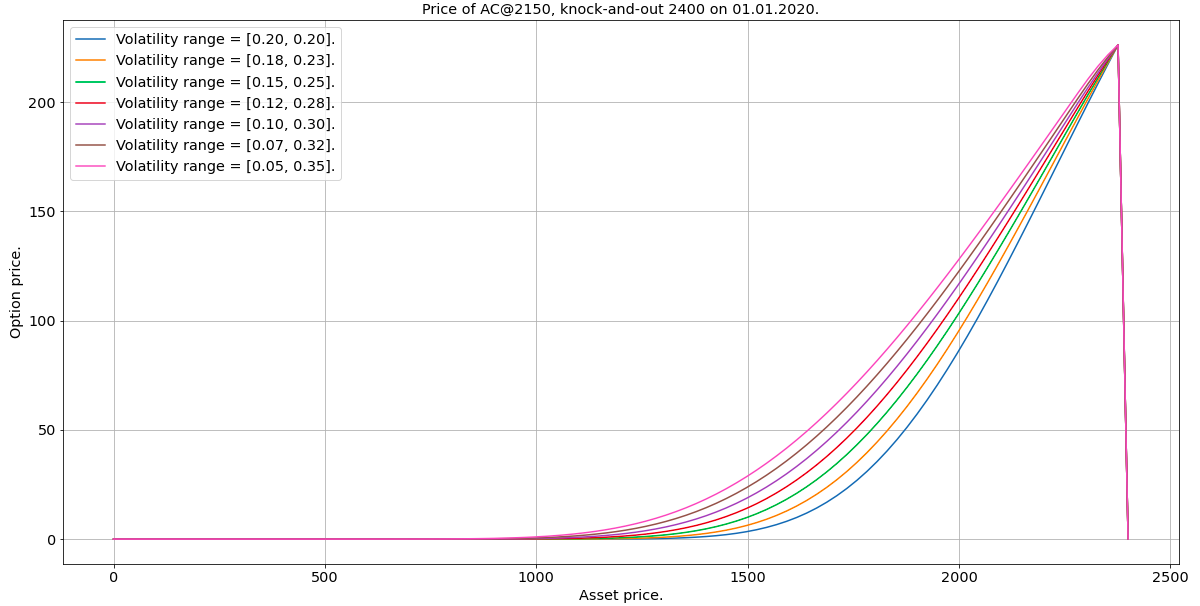
\includegraphics[width=\textwidth,height=\textheight,keepaspectratio]{ac_2150_2400_diff_vol_range.png}
    \caption{Wartość AC@2150, knock-and-out 2400, różne przedziały zmienności.}
    \label{fig:ac_2150_2400_diff_vol_range}
\end{figure}

\begin{figure}[H]
    \centering
    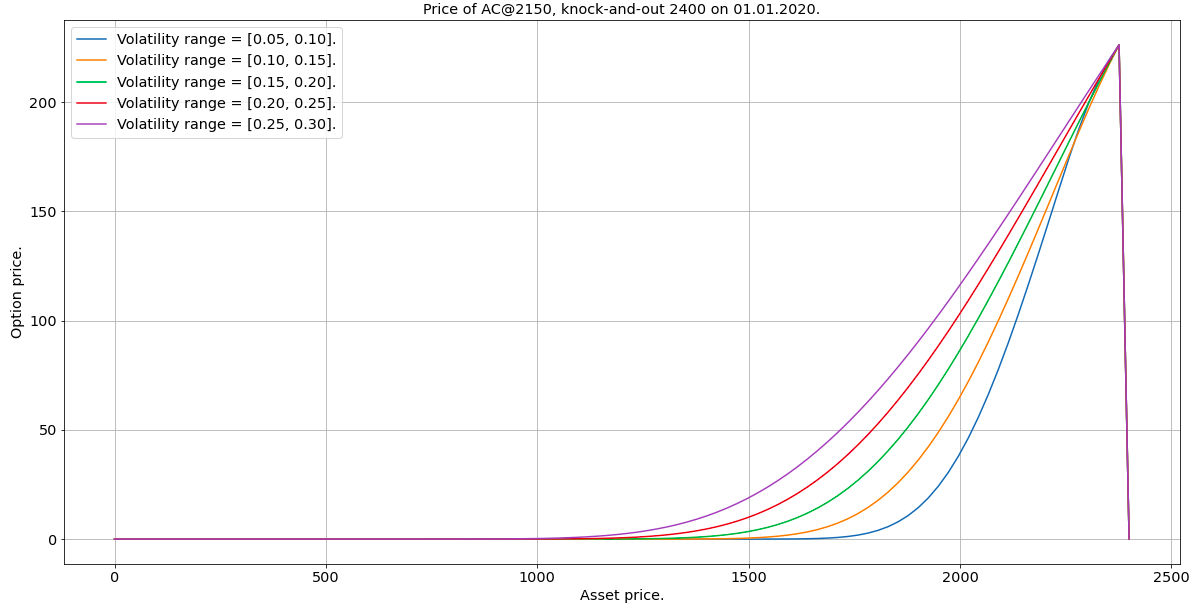
\includegraphics[width=\textwidth,height=\textheight,keepaspectratio]{ac_2150_2400_diff_vol_ex.png}
    \caption{Wartość AC@2150, knock-and-out 2400, różne przedziały zmienności.}
    \label{fig:ac_2150_2400_diff_vol_ex}
\end{figure}

\subsubsection{Momenty wykonania opcji amerykańskich call.}

Wykres \ref{fig:em_ac_2150_2400} przedstawia kiedy powinno się wykonać opcje amerykańską call. Widzimy, że opcję tę powinniśmy wykonać tylko i wyłącznie wtedy gdy jesteśmy na moment przed barierą. 

\begin{figure}[H]
    \centering
    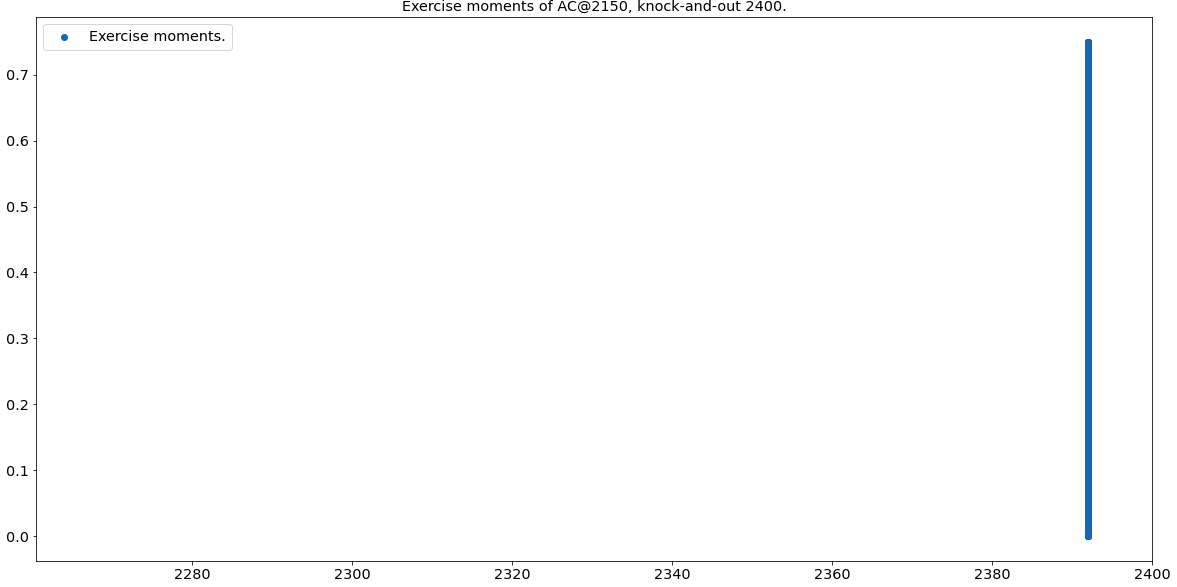
\includegraphics[width=\textwidth,height=\textheight,keepaspectratio]{em_ac_2150_2400.png}
    \caption{Momenty wykonania AC@2150, knock-and-out 2400, $\sigma \in [25\%, 30\%].$}
    \label{fig:em_ac_2150_2400}
\end{figure}

\subsection{Opcje amerykańskie put.}

Poniżej przedstawimy analizę opcji amerykańskich put. 

Wykres \ref{fig:ap_2150_1900_uv} przedstawia wycenę opcji amerykańskiej put z ceną wykonania 2150 i barierą 1900. Obserwujemy sytuację analogiczną do wcześniej rozważanej opcji call. 

\begin{figure}[H]
    \centering
    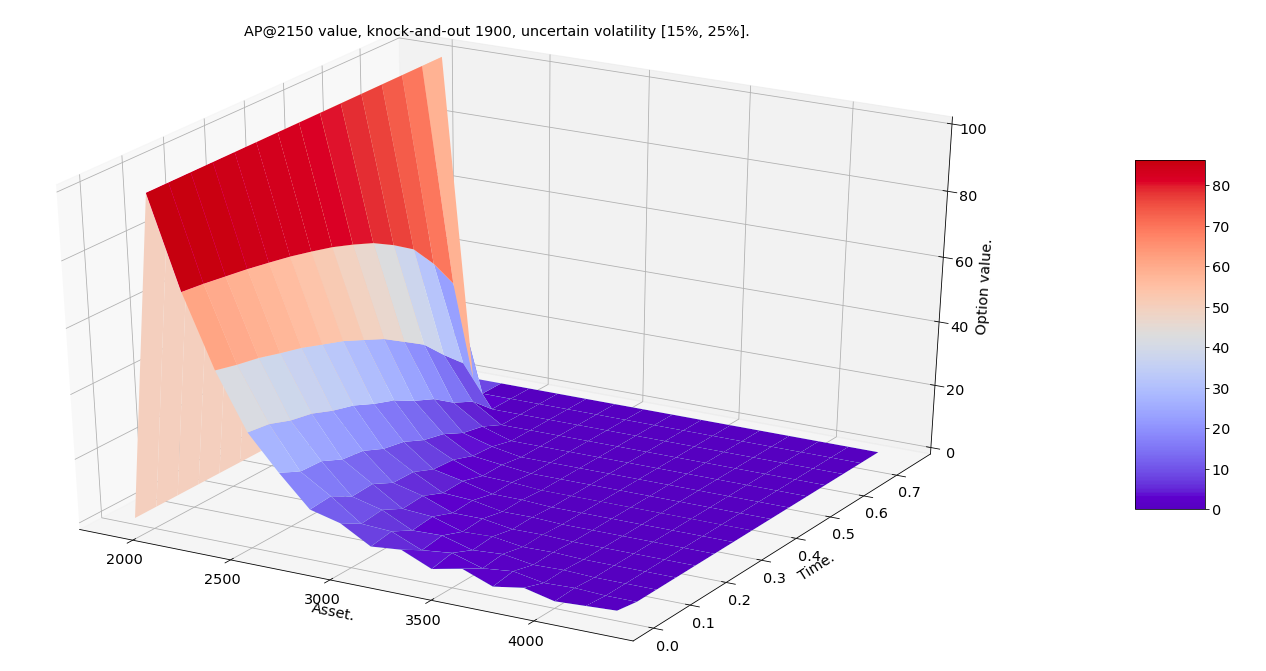
\includegraphics[width=\textwidth,height=\textheight,keepaspectratio]{ap_2150_1900_uv.png}
    \caption{Wartość AC@2150, knock-and-out 2400, różne przedziały zmienności.}
    \label{fig:ap_2150_1900_uv}
\end{figure}

\subsubsection{Momenty wykonania opcji amerykańskich put.}

Wykres \ref{fig:em_ap_2150_1900} przedstawia kiedy powinno się wykonać opcje amerykańską AP@2150, knock-and-out 1900, $\sigma \in [15\%, 25\%].$ Widzimy, że opcję tę powinniśmy wykonać tylko i wyłącznie wtedy gdy jesteśmy na moment przed barierą.  Ciekawszą sytuację mamy, gdy bariera jest bardziej oddalona od ceny wykonania - wykres \ref{fig:em_ap_2150_900}.

\begin{figure}[H]
    \centering
    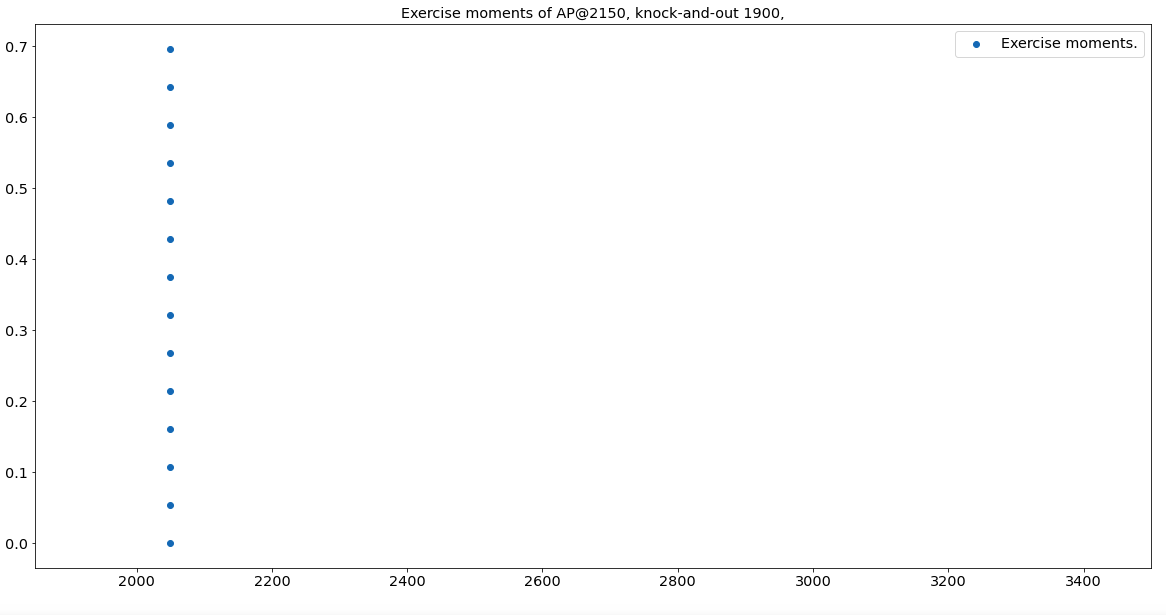
\includegraphics[width=\textwidth,height=\textheight,keepaspectratio]{em_ap_2150_1900.png}
    \caption{Momenty wykonania AP@2150, knock-and-out 1900, $\sigma \in [15\%, 25\%].$}
    \label{fig:em_ap_2150_1900}
\end{figure}

\begin{figure}[H]
    \centering
    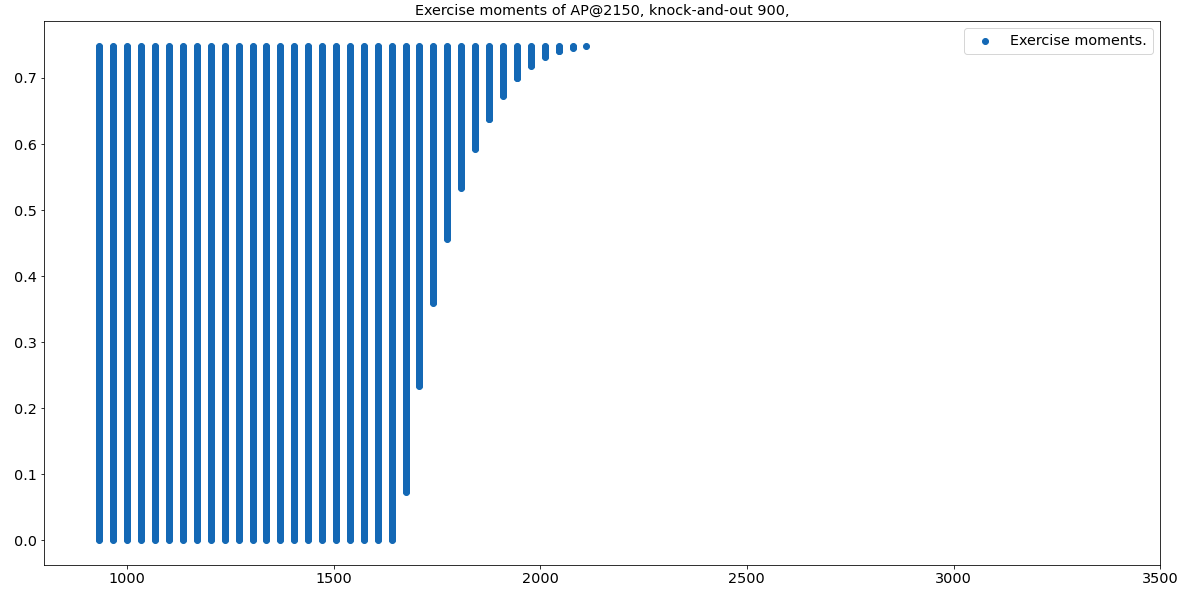
\includegraphics[width=\textwidth,height=\textheight,keepaspectratio]{em_ap_2150_900.png}
    \caption{Momenty wykonania AP@2150, knock-and-out 1900, $\sigma \in [15\%, 25\%].$}
    \label{fig:em_ap_2150_900}
\end{figure}

Poniżej przedstawiamy, jak zmieniają się momenty wykonania przy zmianie przedziału zmienności - wykres \ref{fig:em_ap_2150_900_diff_vol}. Kilka ciekawych obserwacji:
\begin{enumerate}
    \item Im mniejsza zmienność, tym więcej momentów wykonania. 
    \item  Przy $\sigma \in [5\%, 10\%]$, opcję AP@2150, knock-and-out 900 opłaca się wykonać już 1 stycznia jeśli wartość aktywa to co najmniej 2000. 
    \item Tę samą opcję, przy $\sigma \in [30\%, 40\%]$ nie opłaca się wykonać w styczniu nawet jeśli wartość aktywa podstawowego to 1400. 
    \item Widzimy tu 'monotoniczność' momentów wykonania względem zmienności. 
\end{enumerate}

\begin{figure}[H]
    \centering
    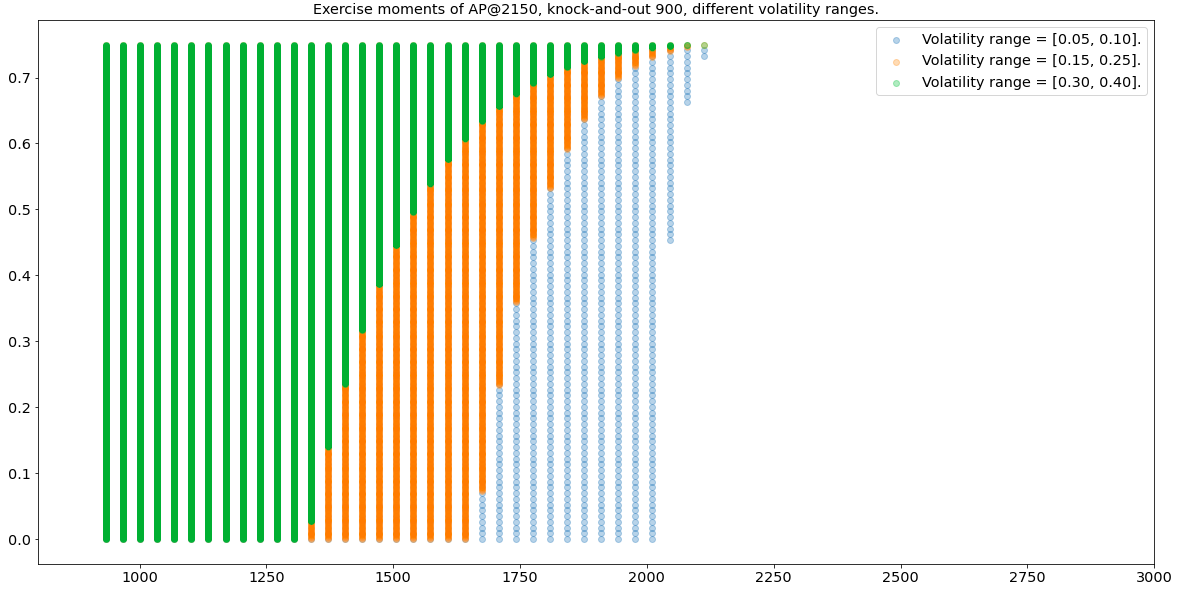
\includegraphics[width=\textwidth,height=\textheight,keepaspectratio]{em_ap_2150_900_diff_vol.png}
    \caption{Momenty wykonania AP@2150, knock-and-out 900, różne przedziały zmienności.}
    \label{fig:em_ap_2150_900_diff_vol}
\end{figure}



\section{Dywidendy}
W tym rozdziale zbadamy wpływ dywidendy procentowej na cenę opcji. Posłużymy się ponownie metodą explicite fine difference, uwzględniającą wypłatę dywidendy. Głównym problemem który nie pozwalał na zwykłe zastosowanie tego algorytmu była zmiana $dS$ (argumentu odpowiadającego za krok po indeksie) w trakcie życia opcji. Rysunek \ref{fig:koncepcja} przedstawia koncepcję rozwiązania tego problemu. 
W poniższych rozważaniach parametry będą wynosić odpowiednio (w przypadku zmiany zostanie to zaznaczone):
\begin{itemize}
    \item zmienność roczna: $[15\%, 25\%]$
    \item cena wykonania: $2150$
    \item moment wypłaty dywidendy: $0.4$
    \item wysokość dywidendy: $0.4$
    \item bariera:
    \begin{itemize}
        \item call: $2400$
        \item put: $1900$
    \end{itemize}
    
\end{itemize}
Wszystkie wykresy trójwymiarowe zaprezentowane w raporcie zostały zamieszczone w załączniku. Dla uproszczenia i skrócenia opcje europejskie barierowe call z dywidendą będą nazywane europejskimi opcjami call, pozostałe przypadki nazwane będą analogicznie.
\begin{figure}[H]
    \centering
    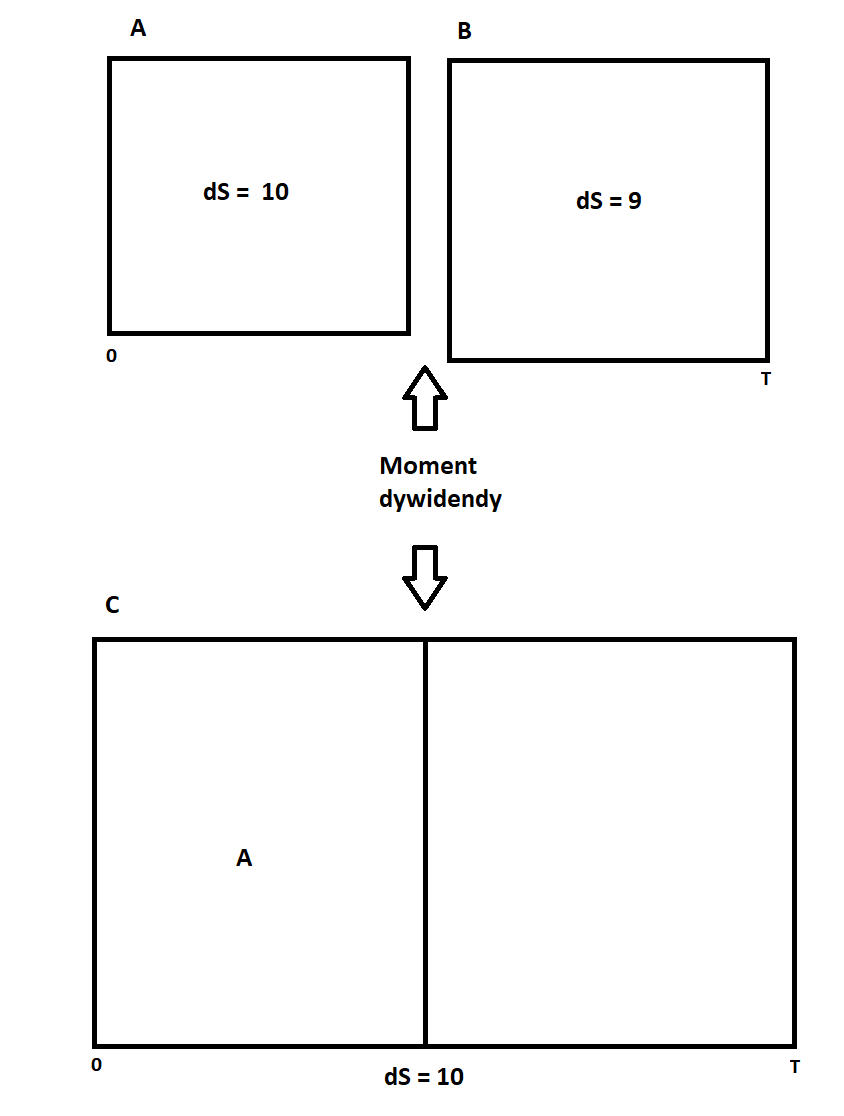
\includegraphics[scale = 0.7]{dividend/koncepcja.png}
    \caption{Schemat przedstawiający modyfikację algorytmu explicite fine difference do wypłaty dywidend procentowych (w przykładzie dywidenda wynosi 10\%, a $dS = 10$). Macierz $B$ wyliczona została przy pomocy niezmodyfikowanego algorytmu dla odpowiednio zmienionego argmendtu $dS$, następnie przy jej pomocy oraz odpowiedniemu przesunięciu indeksu została wyliczona macierz $A$. Kolejnym krokiem było wyliczenie macierzy $C$ z domyślnym krokiem bez uwzględniania dywidendy, a następnie wpisanie wyników z macierzy $A$ do momentu wypłaty dywidendy. Macierz $C$ jest macierzą wynikową.}
    \label{fig:koncepcja}
\end{figure}

\subsection{Opcje europejskie}

\begin{figure}[H]
    \centering
    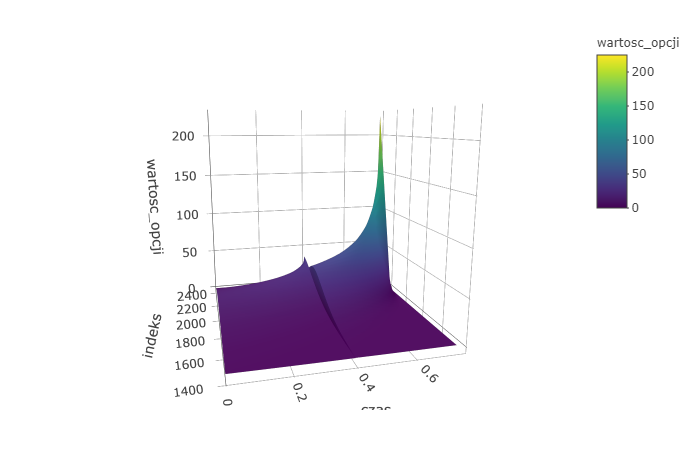
\includegraphics[width=\textwidth,height=\textheight,keepaspectratio]{dividend/call_EU_dywidenda.png}
    \caption{Wartość europejskiej opcji call z dywidendą wypłaconą w czasie $t = 0.4$ w wysokości $10\%$.}
    \label{fig:divi_call_EU}
\end{figure}

Wykres \ref{fig:divi_call_EU} przedstawia wartość europejskiej opcji call z dywidendą wypłaconą w chwili $0.4$. Widać na nim że dywidenda spowodowała przesunięcie w chwili jej wypłaty. Powód tego jest bardzo intuicyjny, jeżeli jesteśmy krótką chwilę przed wypłatą dywidendy i chcielibyśmy kupić opcję to koszt będzie podobny jakbyśmy chwilę po  wypłacie dywidendy kupili tą samą opcję tylko dla adekwatnie zmniejszonego indeksu. Sytuacja z opcją europejską put (przedstawiona na wykresie \ref{fig:divi_put_EU}) wygląda analogicznie jak w przypadku opcji europejskiej call. W chwili wypłaty dywidendy następuje przesunięcie, a powód jego wystąpienia jest taki sam.

\begin{figure}[H]
    \centering
    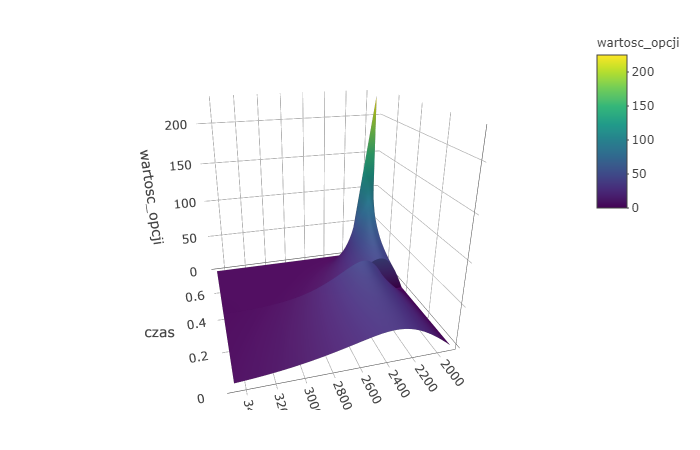
\includegraphics[width=\textwidth,height=\textheight,keepaspectratio]{dividend/put_EU_dywidenda.png}
    \caption{Wartość europejskiej opcji put z dywidendą wypłaconą w czasie $t = 0.4$ w wysokości $10\%$.}
    \label{fig:divi_put_EU}
\end{figure}







\subsection{Opcje amerykańskie}

\begin{figure}[H]
    \centering
    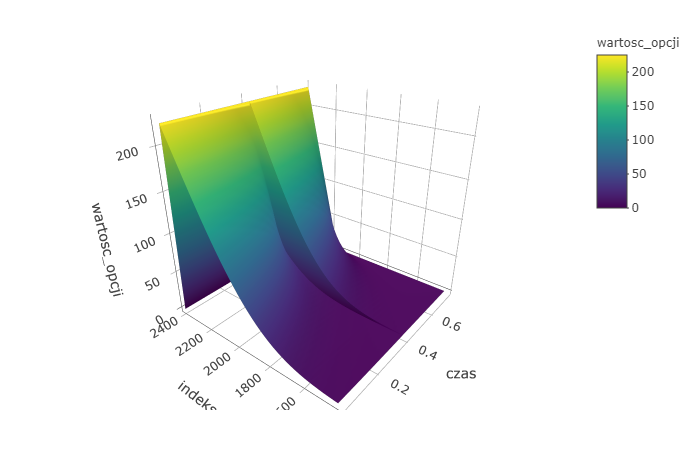
\includegraphics[width=\textwidth,height=\textheight,keepaspectratio]{dividend/call_A_dywidenda.png}
    \caption{Wartość amerykańskiej opcji call z dywidendą wypłaconą w czasie $t = 0.4$ w wysokości $10\%$.}
    \label{fig:divi_call_A}
\end{figure}



\begin{figure}[H]
    \centering
    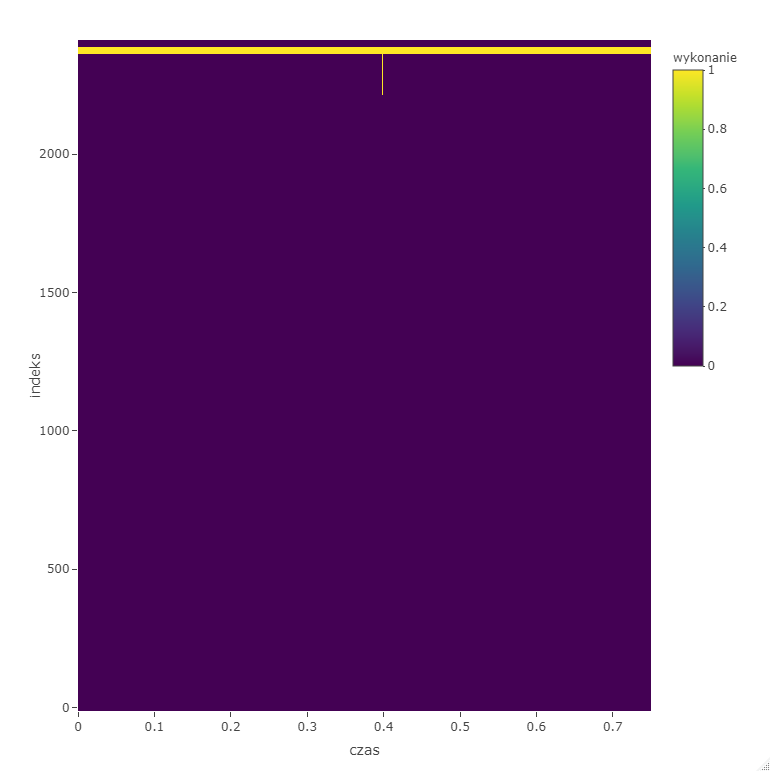
\includegraphics[width=\textwidth,height=\textheight,keepaspectratio]{dividend/wykonanie_call.png}
    \caption{Na żółto zaznaczone są momenty w których opłacalne jest wykonanie amerykańskiej opcji call z wykresu \ref{fig:divi_call_A}.}
    \label{fig:wykonanie_call}
\end{figure}

Na wykresie \ref{fig:divi_call_A} po raz kolejny obserwujemy zmianę ceny w momencie wypłaty dywidendy powód jest dokładnie taki sam jak wcześniej z tym wyjątkiem, że tyczy się to tylko momentów gdzie ,,europejskość" ceny była wyższa niż aktualnego payoffu. Wykres \ref{fig:divi_wysokosc_call_A} przedstawia momenty w których warto wykonać opcję, jak w przypadku wersji bez wypłaty dywidendy opcję opłaca się wykonać tuż przed barierą, oraz w zupełnie nowym miejscu, a dokładnie moment przed wypłatą dywidendy gdy czekanie ,,średnio" daje nam niższy payoff niż aktualny.


\begin{figure}[H]
    \centering
    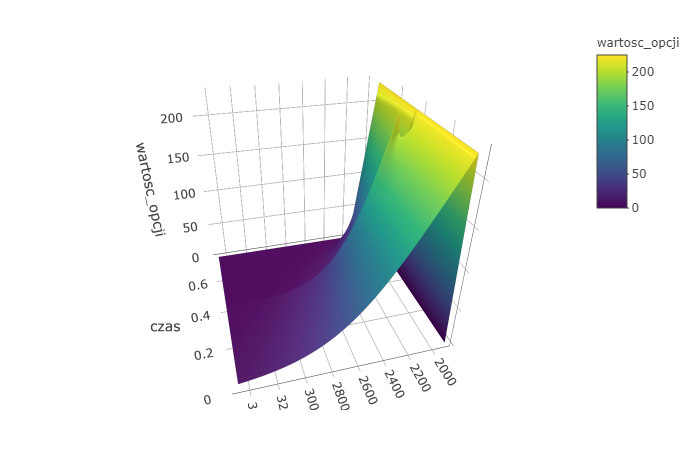
\includegraphics[width=\textwidth,height=\textheight,keepaspectratio]{dividend/put_A_dywidenda.png}
    \caption{Wartość amerykańskiej opcji put z dywidendą wypłaconą w czasie $t = 0.4$ w wysokości $10\%$.}
    \label{fig:divi_put_A}
\end{figure}

\begin{figure}[H]
    \centering
    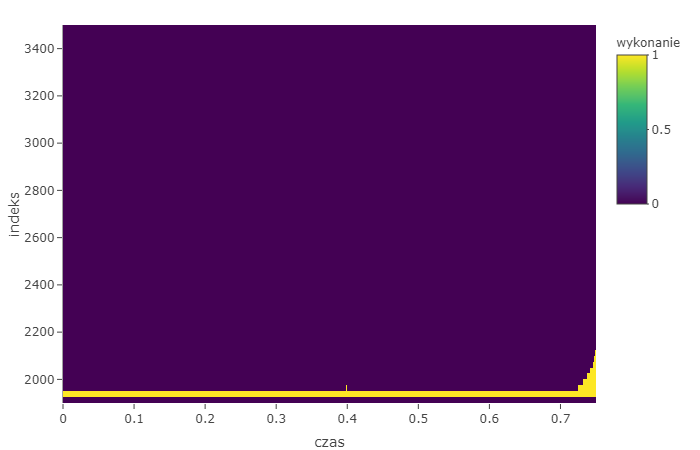
\includegraphics[width=\textwidth,height=\textheight,keepaspectratio]{dividend/wykonanie_put.png}
    \caption{Na żółto zaznaczone są momenty w których opłacalne jest wykonanie amerykańskiej opcji put z wykresu \ref{fig:divi_put_A}.}
    \label{fig:wykonanie_put}
\end{figure}


W przypadku opcji put sytuacja znowu wygląda analogicznie jak w call, jednak w odróżnieniu do tej drugiej opcja sprzedaży zyskuje na niskiej wartości indeksu. W rezultacie przed dywidendą w okolicy wartości indeksu równej $2200$ pojawia się ,,cypel" związany jest on z tym, że ,,europejskość" jest znacznie wyższa od aktualnego payoffu, tzn bardziej opłaca nam się czekać niż wykonać opcję w chwili obecnej. I rzeczywiście po wypłaceniu dywidendy znajdziemy się w miejscu bliskim maksymalnego payoffu. Natomiast wraz ze spadkiem wartości indeksu, dywidenda powoduje że w następnym kroku uderzamy w barierę. Z tego powodu wykonanie opcji jest w tym miejscu bardziej opłacalne (sytuację ilustruje wykres \ref{fig:wykonanie_put}), różnica wartości oczekiwanej z przyszłości z aktualnym payoffem, powoduje charakterystyczny skok nazwany wcześniej ,, cypelkiem".

\begin{figure}[H]
    \centering
    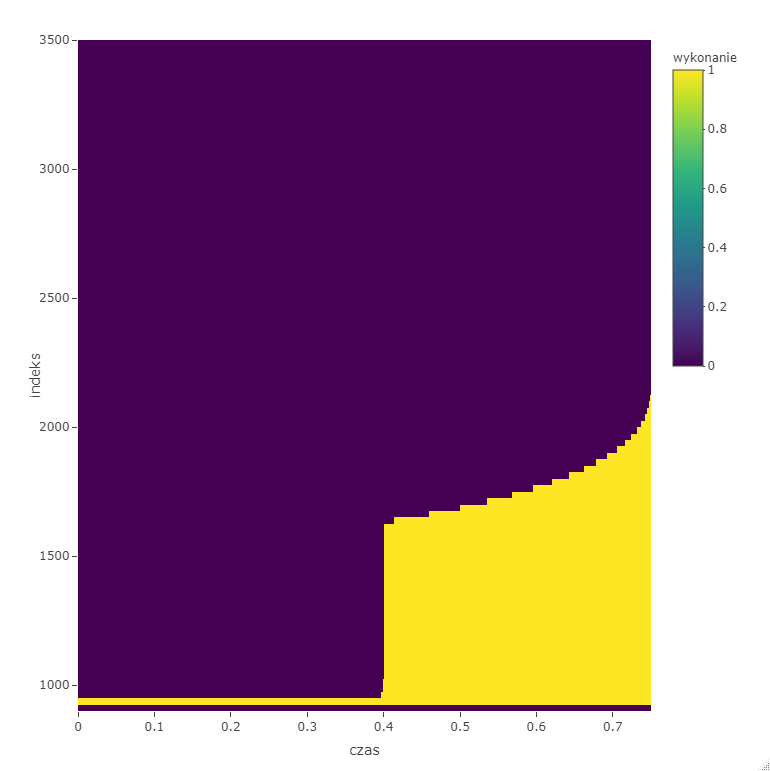
\includegraphics[width=\textwidth,height=\textheight,keepaspectratio]{dividend/wykonanie_put_900.png}
    \caption{Na żółto zaznaczone są momenty w których opłacalne jest wykonanie amerykańskiej opcji call z barierą równą 900.}
    \label{fig:divi_put_EU_900}
\end{figure}
Postanowiliśmy porównać momenty wykonania dla bariery równej $900$ (jak w przypadku opcji bez dywidendy; wykres \ref{fig:em_ap_2150_900}). Z wykresu \ref{fig:divi_put_EU_900} można odczytać, że wykonanie opcji przed wypłatą dywidendy jest nieopłacalne. Oczywiście wyjątkiem od tej reguły są miejsca kiedy wartość indeksu znajduje się przy barierze, albo gdy dywidenda spowoduje że uderzymy w barierę.

\subsection{Wpływ parametrów}

W tym rozdziale skupimy się na zmianie parametrów odpowiadających za wypłątę dywidendy.

\subsubsection{Moment wypłaty dywidendy}

\begin{figure}[H]
    \centering
    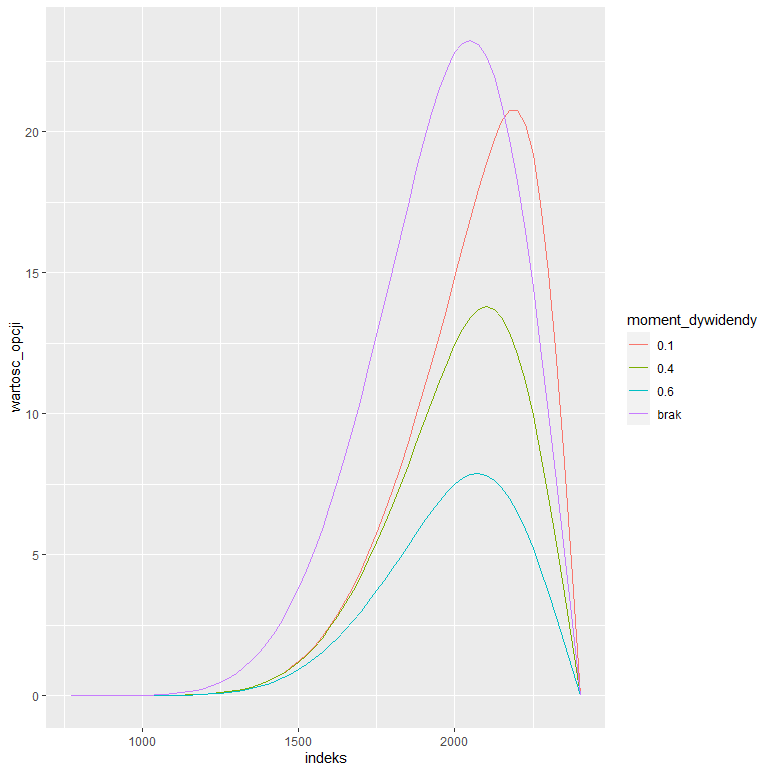
\includegraphics[width=\textwidth,height=\textheight,keepaspectratio]{dividend/call_EU_procent_moment_dywidendy.png}
    \caption{Cena opcji call europejskiej ze względu na moment zapadania dywidendy}
    \label{fig:moment_call_EU}
\end{figure}

Moment wypłaty dywidendy ma spory wpływ na wycenę opcji. Wykres \ref{fig:moment_call_EU} przedstawia wartość opcji europejskiej call, ze względu na moment wypłacenia dywidendy. Oczywisty jest fakt, że dla większości przypadków dywidenda spowoduje spadek cen opcji, jedynie sytuacja w której mamy dużą szansę uderzenia w barierę oraz stosunkowo szybkie wykonanie dywidendy, zwiększa nam cenę. Wraz z późniejszym wykonaniem dywidendy maleje cena opcji, wiąże się to z dość oczywistym faktem, iż szansa na uderzenie w barierę rośnie, wiąże się to z ograniczeniem wysokości payoffu (im później zostanie wykonana dywidenda tym mamy mniejszą szansę na wysoki payoff). Natomiast w przypadku opcji amerykańskiej call, obserwujemy odwrotną tendencję (wykres \ref{fig:moment_call_A}) spowodowane jest to poprzez krótszy okres w którym mamy szansę na wykonanie opcji przed samą barierą ( warto zwrócić w tym momencie uwagę na fakt, że wartości opcji o różnych momentach wypłaty dywidend, są równe od momentu wypłaty ostatniej dywidendy).

\begin{figure}[H]
    \centering
    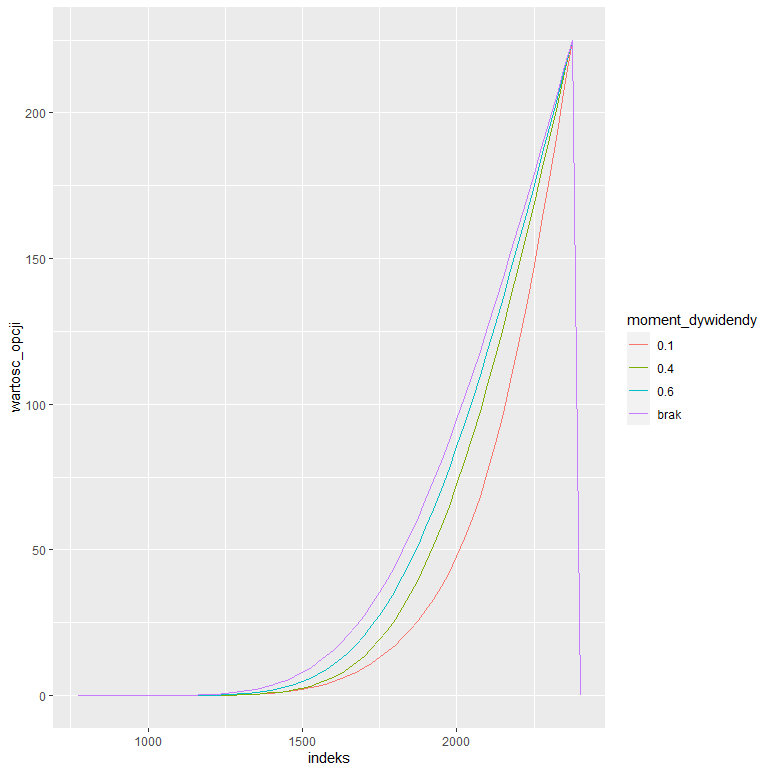
\includegraphics[width=\textwidth,height=\textheight,keepaspectratio]{dividend/call_A_procent_moment_dywidendy.png}
    \caption{Cena opcji call amerykańskiej ze względu na moment wypłaty dywidendy.}
    \label{fig:moment_call_A}
\end{figure}

\begin{figure}[H]
    \centering
    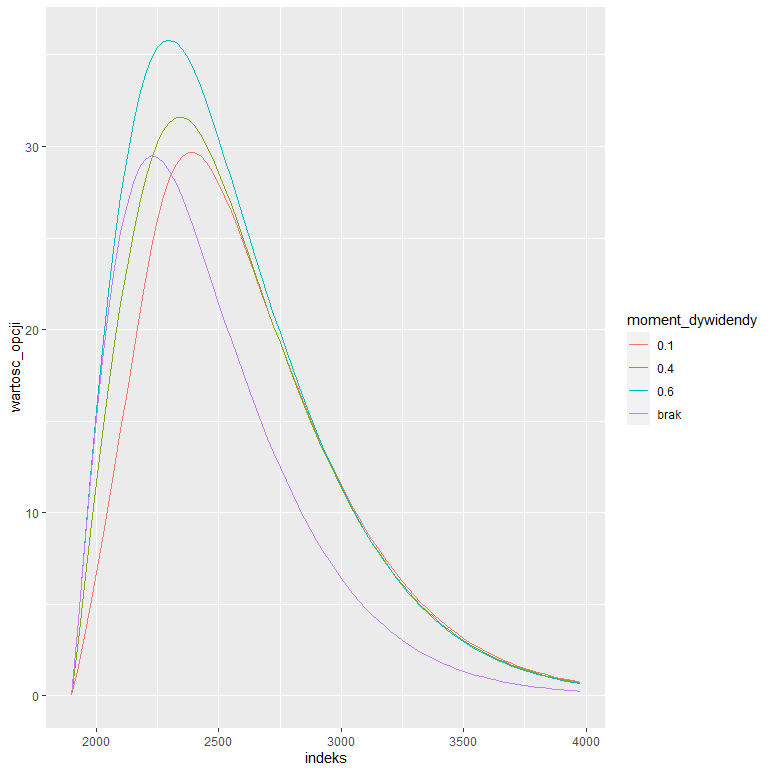
\includegraphics[width=\textwidth,height=\textheight,keepaspectratio]{dividend/put_EU_procent_moment_dywidendy.png}
    \caption{Cena opcji put europejskiej ze względu na moment zapadania dywidendy}
    \label{fig:moment_put_EU}
\end{figure}

W przypadku opcji put sytuacja wygląda, odwrotnie wraz z opóźnianiem wypłaty dywidendy rośnie cena opcji, analogicznie późniejsza dywidenda zmniejsza szansę na uderzenie w barierę. Z kolei w przypadku amerykańskiej opcji put (wykres \ref{fig:moment_put_A}), szybsza wypłata dywidendy powoduje że będziemy mieć większą szansę do przedwczesnego wykonania opcji (czyli uzyskania optymalnego payoffu). Przy zbyt wczesnej wypłacie dywidendy ($t_d = 0.1$) w pewnym momencie widać ,,naleciałość europejskości" która, jak już wcześniej wspominaliśmy była w pewnym momencie znacznie wyższa od payoffu (,,cypelek").




\begin{figure}[H]
    \centering
    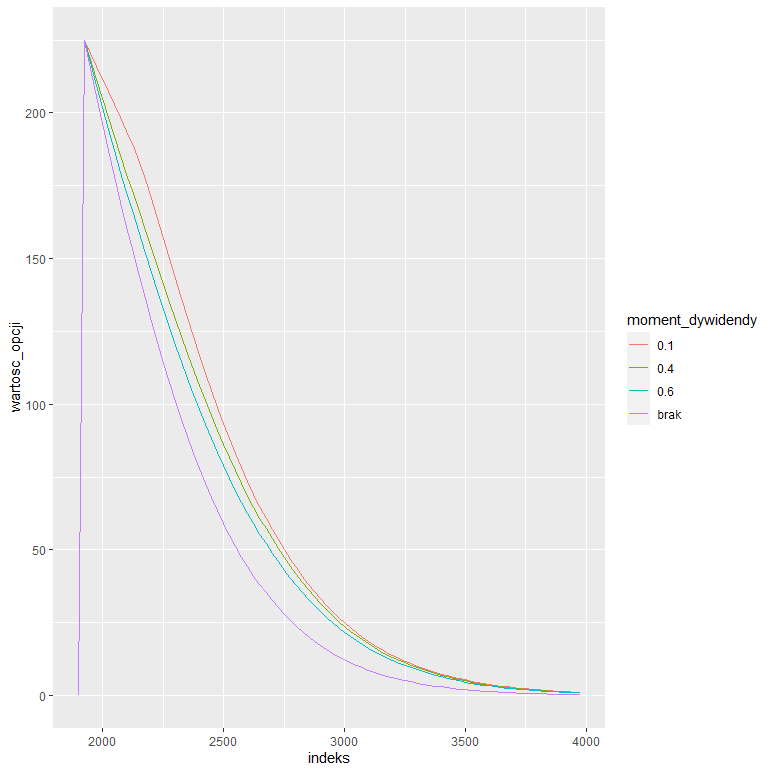
\includegraphics[width=\textwidth,height=\textheight,keepaspectratio]{dividend/put_A_procent_moment_dywidendy.png}
    \caption{Cena opcji put amerykańskiej ze względu na moment wypłaty dywidendy.}
    \label{fig:moment_put_A}
\end{figure}



\subsubsection{Zmiana wysokości dywidendy}

Zmiana wysokości dywidendy w przypadku opcji call europejskiej (wykres \ref{fig:divi_wysokosc_call_EU}) oraz amerykańskiej (wykres \ref{fig:divi_wysokosc_call_A}) powoduje, że ceny akcji spadają wraz z wzrostem dywidendy, fakt ten jest oczywisty i nie wymaga komentarza.

\begin{figure}[H]
    \centering
    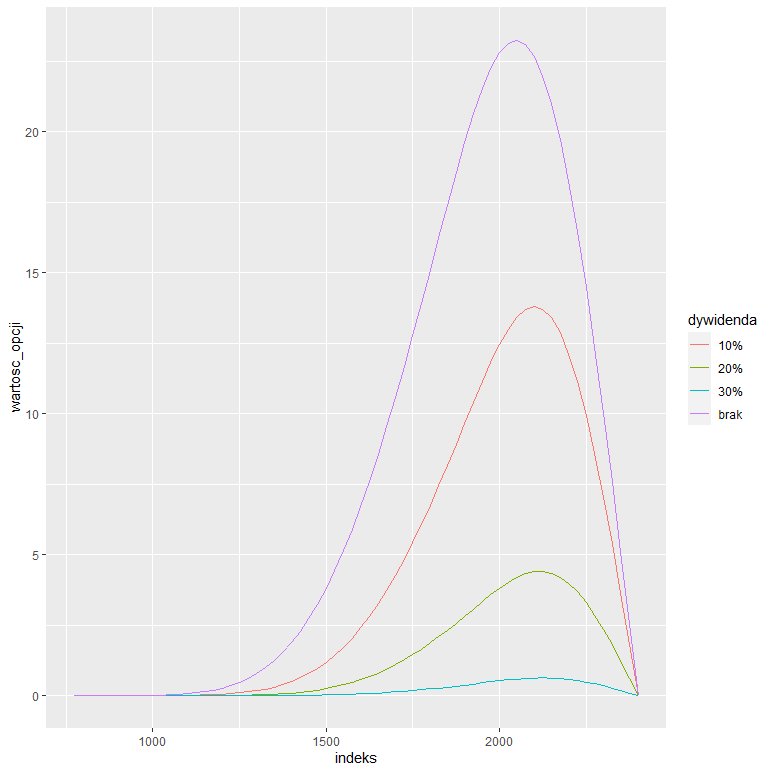
\includegraphics[width=\textwidth,height=\textheight,keepaspectratio]{dividend/zmiennosc_dywidendy_call_EU.png}
    \caption{Cena opcji call europejskiej ze względu na wysokość dywidendy}
    \label{fig:divi_wysokosc_call_EU}
\end{figure}

\begin{figure}[H]
    \centering
    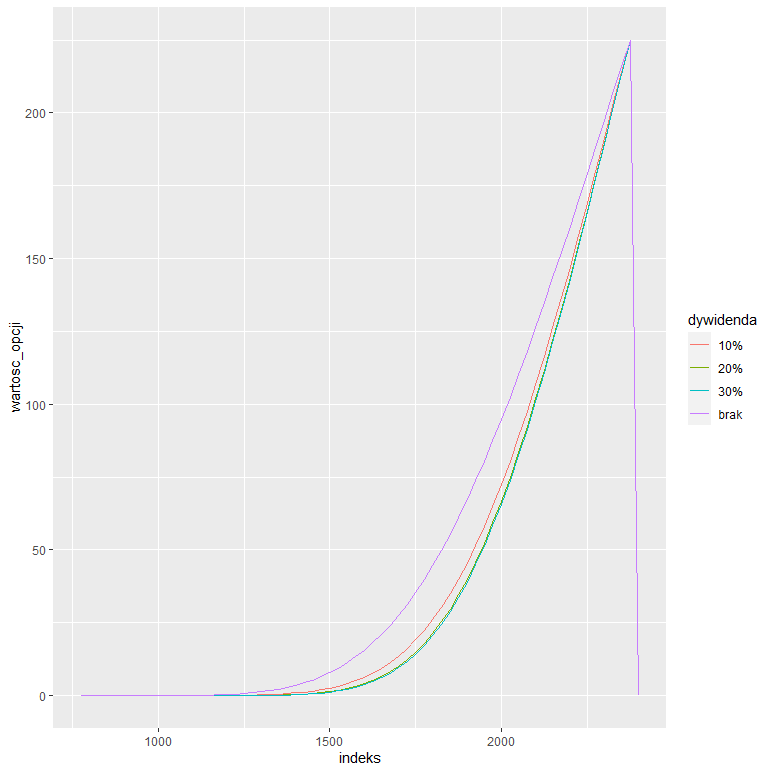
\includegraphics[width=\textwidth,height=\textheight,keepaspectratio]{dividend/zmiennosc_dywidendy_call_A.png}
    \caption{Cena opcji call amerykańskiej ze względu na wysokość dywidendy}
    \label{fig:divi_wysokosc_call_A}
\end{figure}

Ciekawą sytuację można zaobserwować w przypadku opcji europejskiej put przedstawionej na wykresie \ref{fig:divi_wysokosc_put_EU}. Wraz z wzrostem dywidendy, maksymalna cena opcji przyjmowana jest dla coraz większych wartości indeksu oraz nieznacznie rośnie. Pierwszą własność łatwo wytłumaczyć, jest ona konsekwencją zmiany wartości indeksu w momencie wypłaty dywidendy. Jeżeli odległość od bariery jest zbyt niska, uderzymy w nią. W przypadku opcji amerykańskiej sytuacja się nieco komplikuje dla dywidend $10\%$ oraz $20\%$ wykres zachowuje się przewidywalnie, czyli cena rośnie wraz z wzrostem dywidendy. Wysoka dywidenda, w postaci $30\%$ wypłaty, zmienia jednak to zachowanie. Przed wypłatą dywidendy ,,cypelek" zmienia się w ,,górę" co obrazuje wykres \ref{fig:divi_30}. Tak duża zmiana w cenie indeksu, przy tak niewielkiej zmianie czasu, powoduje że dla zbyt niskich wartości aktywa, opcja zachowuje się bardzo podobnie do opcji w której nie wystąpi dywidenda. Natomiast od pewnego momentu dywidenda zaczyna ,,obiecywać" wysoki zysk pomimo faktu, że payoff w tych miejscach jest równy $0$. Oczywiście tak wysokie dywidendy nie występują na rynku, więc ta anomalia jest jedynie ciekawostką.
\begin{figure}[H]
    \centering
    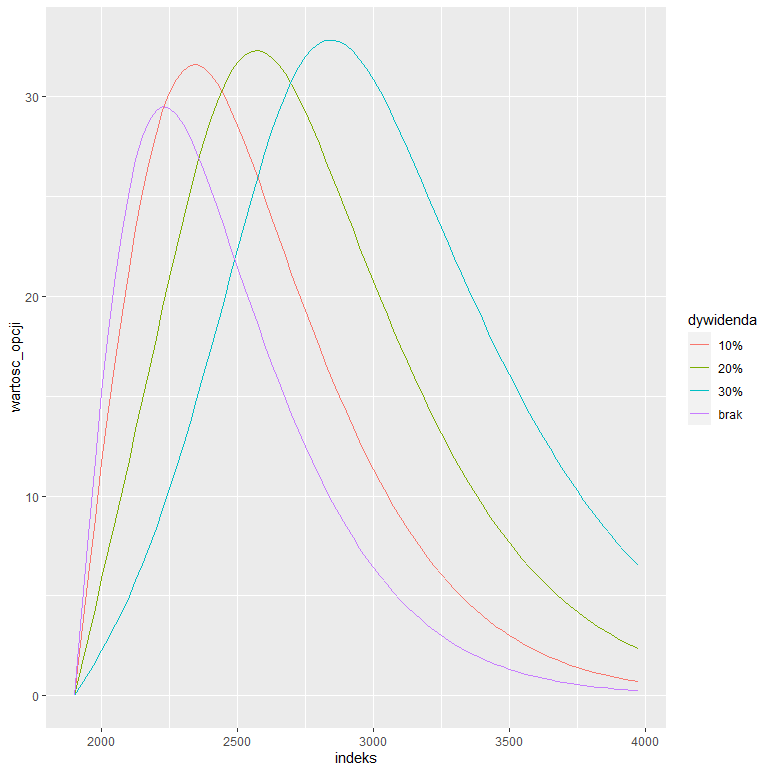
\includegraphics[width=\textwidth,height=\textheight,keepaspectratio]{dividend/zmiennosc_dywidendy_put_EU.png}
    \caption{Cena opcji put europejskiej ze względu na wysokość dywidendy}
    \label{fig:divi_wysokosc_put_EU}
\end{figure}





\begin{figure}[H]
    \centering
    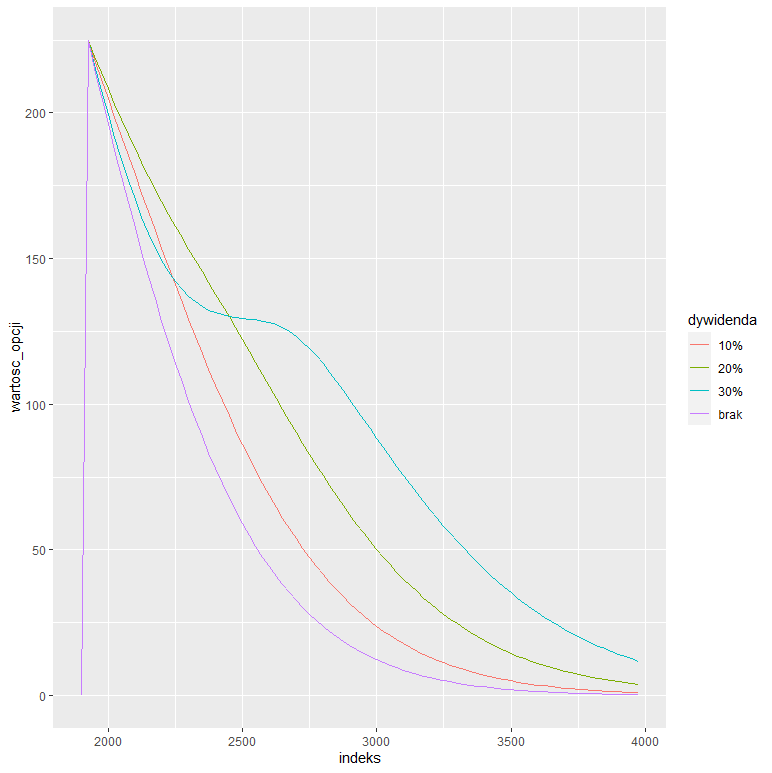
\includegraphics[width=\textwidth,height=\textheight,keepaspectratio]{dividend/zmiennosc_dywidendy_put_A.png}
    \caption{Amerykańska opcja put z dywidendą $30\%$}
    \label{fig:divi_30}
\end{figure}

\begin{figure}[H]
    \centering
    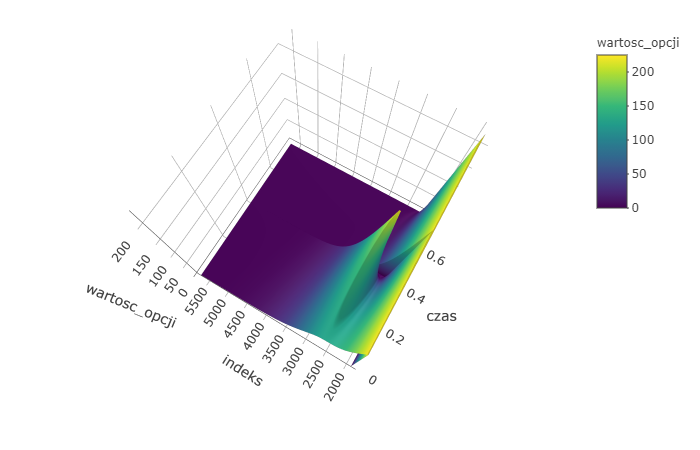
\includegraphics[width=\textwidth,height=\textheight,keepaspectratio]{dividend/dywidenda_30.png}
    \caption{Cena opcji put amerykańskiej ze względu na wysokość dywidendy}
    \label{fig:divi_wysokosc_put_A}
\end{figure}


Zaimplementowaliśmy również dywidendy kwotowe jednakże przy odpowiednim doborze parametrów otrzymaliśmy zbliżone wykresy co wiązało się z identycznymi wnioskami. Z tego powodu nie znalazły się w raporcie.



\section{Sprawdzenie wyników}
Metoda finite-difference jest uznaną i sprawdzoną metodą wyceny opcji, ale zawsze istnieje szansa, że podczas implementacji popełniliśmy błąd. Aby nabrać przekonania co do prawdziwości otrzymanych wyników możemy użyć innych znanych nam metod wyceny, które może nie będą działały w takiej ogólności jak finite-difference, ale za to są nieco łatwiejsze w implementacji.

Wybrane metody wyceny opcji:
\begin{enumerate}
    \item Jawne wzory (spełniające równanie Blacka-Scholesa): istnieją dla europejskich opcji barierowych,
    \item Drzewo trójmianowe: metoda pozwala wycenić barierowe opcje europejskie i amerykańskie (możliwość wprowadzenia dywidendy procentowej),
    \item Metoda Monte Carlo: w swej podstawowej formie nadaje się do wyceny europejskich opcji barierowych z dywidendą procentową bądź kwotową.
\end{enumerate}

Należy zauważyć, że powyższe metody nie dają nam od razu całej siatki wyceny opcji, a jedynie jej wartość w chwili zero dla konkretnej wartości początkowej aktywa bazowego. Innym zaletą finite-difference jest możliwość wprowadzenia do modelu niepewnej zmienności, na co nie pozwalają pozostałe metody.

\subsection{Drzewo trójmianowe}

Model wyceny opcji barierowych za pomocą drzewa trójmianowego jest naturalnym rozszerzeniem metody drzewa dwumianowego. W tym wypadku zakładamy, że w każdym kroku czasu \(dt\) cena aktywa bazowego wykonuje albo skok do góry, albo w dół, albo pozostaje na tym samym poziomie. Wysokość skoków dobieramy zgodnie ze zmiennością i wielkością \(dt\) oraz tak aby bariera wypadła na jednym z poziomów cen aktywa (patrz Rysunek \ref{fig:tbt}). W ten sposób zapewniamy, że bariera stosowana podczas wyceny jest dokładnie taka jak ta zadana. 

\begin{figure}[H]
    \centering
    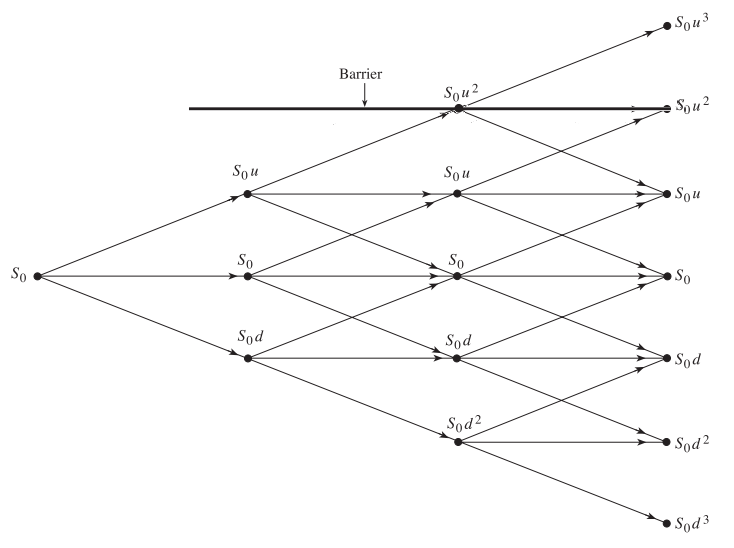
\includegraphics[width=0.75\textwidth,height=\textheight,keepaspectratio]{tbt.png}
    \caption{Drzewo trójmianowe}
    \label{fig:tbt}
\end{figure}

Prawdopodobieństwa przejść są tak dobrane aby ruchy cen akcji odpowiadały światowi neutralnemu na ryzyko. Wyceny dokonujemy dla kolejnych kolumn drzewa (podążając z prawej do lewej) w każdym wierzchołku wpisując wartość opcji odpowiadającą temu wierzchołkowi wyliczoną jako zdyskontowana wartość oczekiwana opcji w następnym kroku. 

Warto zauważyć, że łatwo możemy wprowadzić w tym modelu dywidendę procentową (ceny aktywa zaliczą spadek w momencie dywidendy), ale nie kwotową, ponieważ taki spadek spowoduje, że wierzchołki drzewa przestaną się rekombinować (sklejać) po momencie dywidendy.

\subsection{Opcje europejskie i amerykańskie bez dywidendy}

Dla ustalenia uwagi w tym rozdziale, jeśli nie zostanie stwierdzone inaczej będziemy rozważać następujące parametry opcji: 
\begin{itemize}
    \item cena wykonania: \(2100\),
    \item bariera dla opcji call: \(2400\),
    \item bariera dla opcji put: \(1900\),
    \item zmienność roczna: \(20\%\),
    \item stopa procentowa: \(1.5\%\).
\end{itemize}

Dokonujemy wyceny opcji na chwilę zero dla różnych wartości początkowych aktywa bazowego (\(S_{0}\)).

\begin{figure}[H]
    \centering
    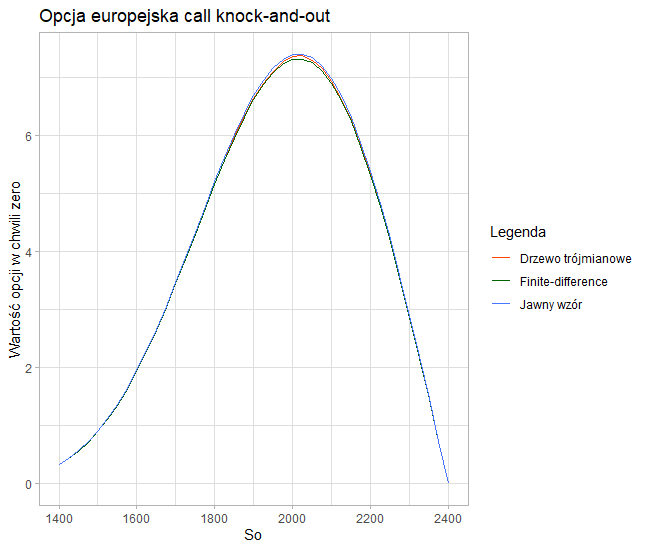
\includegraphics[width=0.8\textwidth,height=\textheight,keepaspectratio]{ec_porownanie.png}
    %\caption{Drzewo trójmianowe}
    \label{fig:ec}
\end{figure}

\begin{figure}[H]
    \centering
    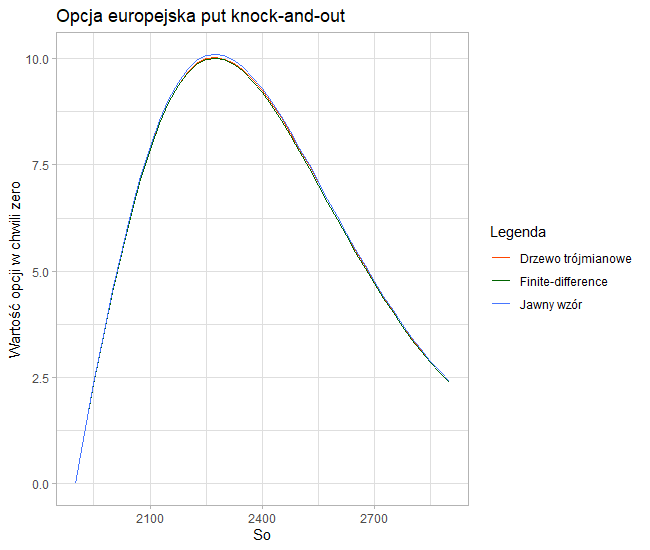
\includegraphics[width=0.8\textwidth,height=\textheight,keepaspectratio]{ep_porownanie.png}
    %\caption{Drzewo trójmianowe}
    \label{fig:ep}
\end{figure}

\begin{figure}[H]
    \centering
    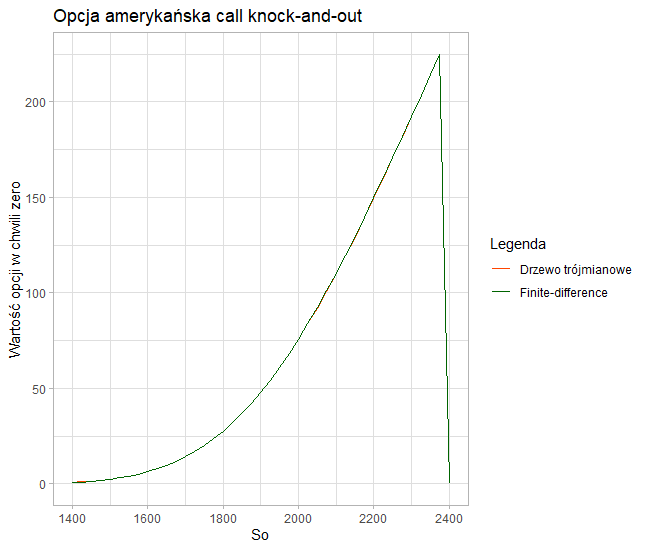
\includegraphics[width=0.8\textwidth,height=\textheight,keepaspectratio]{ac_porownanie.png}
    %\caption{Drzewo trójmianowe}
    \label{fig:ac}
\end{figure}

\begin{figure}[H]
    \centering
    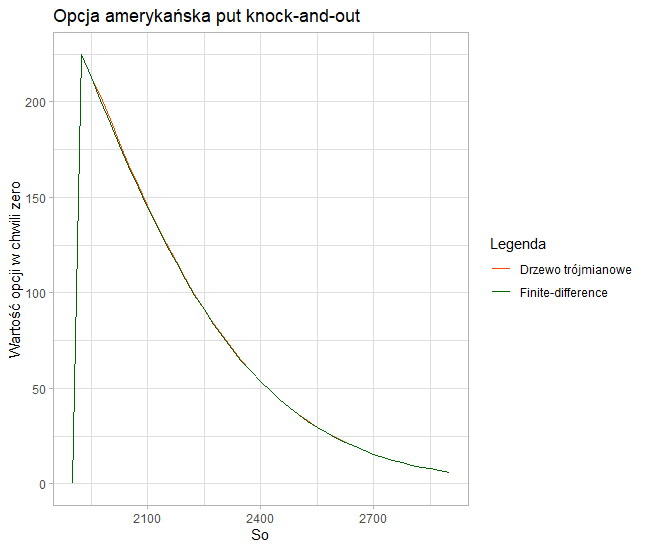
\includegraphics[width=0.8\textwidth,height=\textheight,keepaspectratio]{ap_porownanie.png}
    %\caption{Drzewo trójmianowe}
    \label{fig:ap}
\end{figure}

\begin{tabular}{c||c|c|c|c}
    Rodzaj opcji & EC & EP & AC & AP \\
    \hline
    Maksymalna różnica & 0.086 & 0.095 & 0.37 & 2.65
\end{tabular}\\

Widzimy, że nasze wyceny pokrywają się niemal idealnie. Oczywiście pokazaliśmy zgodność tylko dla jakichś przykładowych parametrów, ale szansa, że to nam się udało przez przypadek jest raczej znikoma. \\

Ważnym parametrem podczas wyceny była zmienność. Możemy zatem popatrzeć na wyceny opcji dla różnych wartości zmienności. Niech \(S_{0}\) dla opcji call wynosi \(2000\), a dla opcji put - \(2400\).

\begin{figure}[H]
    \centering
    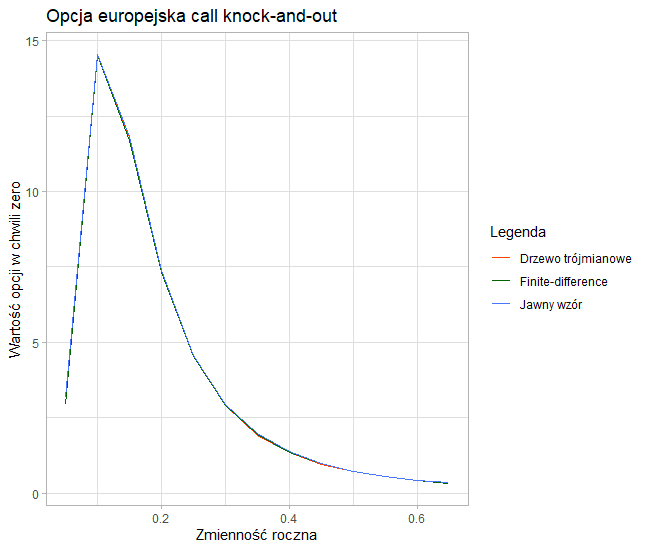
\includegraphics[width=0.8\textwidth,height=\textheight,keepaspectratio]{ec_sig_porownanie.png}
    %\caption{Drzewo trójmianowe}
    \label{fig:ecs}
\end{figure}

\begin{figure}[H]
    \centering
    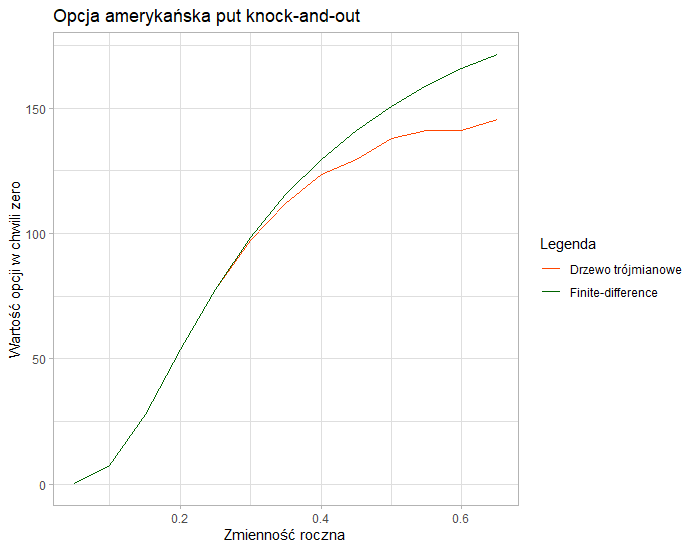
\includegraphics[width=0.8\textwidth,height=\textheight,keepaspectratio]{ap_sigma.png}
    %\caption{Drzewo trójmianowe}
    \label{fig:aps}
\end{figure}

Ponownie obserwujemy zgodność wycen. Jedyna rozbieżność zaczyna pojawiać się dla opcji amerykańskiej z wysoką zmiennością. Jest to spowodowane za małą liczbą kroków przy wycenie drzewem trójmianowym. Większa zmienność przekłada się na większe skoki cen aktywa, przez co następuje niedoszacowanie wartości opcji amerykańskiej (możliwość wczesnego wykonania tuż przed barierą). Zwiększenie liczby kroków w algorytmie powoduje zbliżenie się wyceny do finite-difference (w zamian algorytm staje się powolny).

\subsection{Metoda Monte Carlo}

Wartość opcji może być wyznaczona jako zdyskontowana wartość oczekiwana payoffu, jeśli trajektorie kursu aktywa będą modelowane przez geometryczny ruch Browna w świecie neutralnym na ryzyko, tzn. będą spełniały: \[dS=rSdt+\sigma SdX,\] gdzie \(X\) jest standardowym ruchem Browna. Wartość opcji wynosi wtedy: \[f=e^{-rT}E[payoff(S)].\]

Metoda Monte Carlo polega więc na tym, aby wygenerować \(M\) takich trajektorii obliczyć ich payoffy, wyciągnąć średnią i ją zdyskontować. Mocne Prawo Wielkich Liczb mówi nam, że tak otrzymana wartość \(\mu\) opcji będzie zbiegać do \(f\), gdy \(M\rightarrow \infty\). 

Ponadto możemy wyznaczyć przedział ufności, w którym \(f\) znajdzie się z prawdopodobieństwem \(95\%\): \[\Big( \mu - \frac{1.96\omega}{\sqrt{M}},\, \mu + \frac{1.96\omega}{\sqrt{M}}\Big),\] gdzie \(\omega\) jest odchyleniem standardowym z otrzymanych payoffów.

Metoda ta jest bardzo prosta w użyciu i łatwa w modyfikacji (np. wprowadzenie dywidendy), ciężej jest ją dostosować do wyceny opcji amerykańskich (nie będziemy tego robić). Największym mankamentem jest konieczność wygenerowania bardzo wielu trajektorii, aby uzyskać sensowny przedział ufności.

\subsection{Opcje z dywidendą}
W tym rozdziale zakładamy, że dywidenda jest wypłacana w połowie życia opcji.\\

W metodzie Monte Carlo generowaliśmy \(M=50000\) trajektorii, co dawało przedziały ufności (na poziomie istotności \(\alpha=0.05\)) nie dłuższe niż \(0.6\).

\begin{figure}[H]
    \centering
    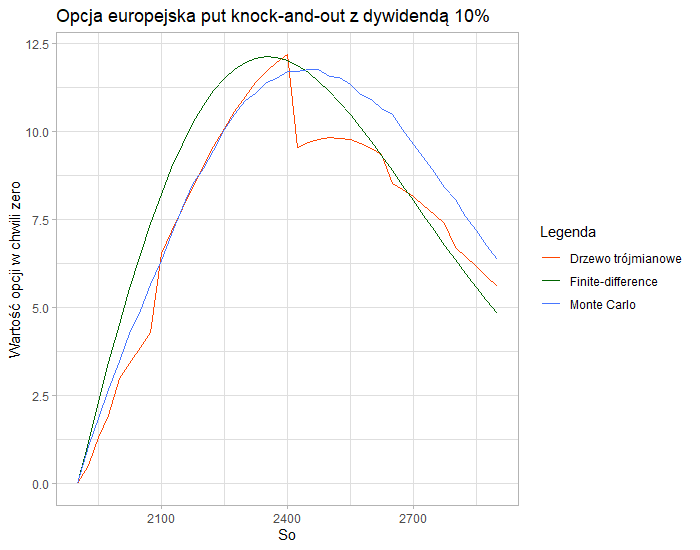
\includegraphics[width=0.8\textwidth,height=\textheight,keepaspectratio]{dyw10proc.png}
    \caption{}
    \label{d10}
\end{figure}

Na Rysunku \ref{d10} mamy przedstawioną wycenę opcji europejskiej put z dywidendą procentową trzema metodami. Choć nie pokrywają się już tak idealnie jak poprzednio, to nadal są to bardzo zbliżone wyceny. Widać jednak, że dywidenda wprowadziła dosyć gwałtowną zmianę w procesie wyceny, z którą różne metody różnie sobie poradziły. Zauważmy na przykład, że bariera w drzewie trójmianowym po momencie dywidendy nie musi już leżeć nie jakimś poziomie cen aktywa, na czym nam zależało.

\begin{figure}[H]
    \centering
    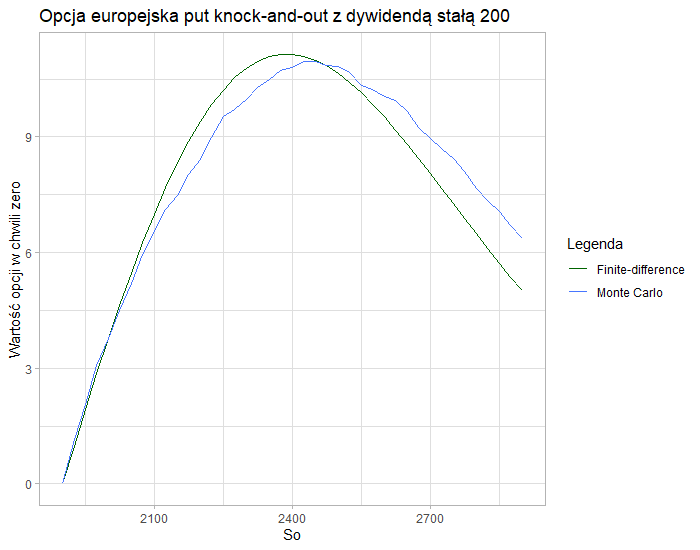
\includegraphics[width=0.8\textwidth,height=\textheight,keepaspectratio]{dyw200.png}
    \caption{}
    \label{d200}
\end{figure}

\begin{figure}[H]
    \centering
    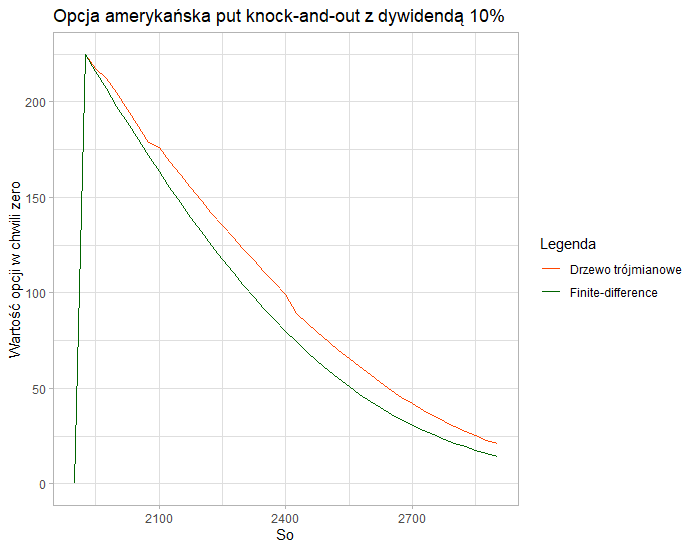
\includegraphics[width=0.8\textwidth,height=\textheight,keepaspectratio]{ap_dyw10.png}
    \caption{}
    \label{adyw}
\end{figure}

Rysunek \ref{d200} przedstawia porównanie dla dywidendy kwotowej, a Rysunek \ref{adyw} dla opcji amerykańskiej. Są to ponownie bardzo zbliżone wyniki. Niestety nie posiadamy zaimplementowanej metody, kora pomogłaby nam sprawdzić wycenę finite-difference opcji amerykańskiej z dywidendą kwotową.

\subsection{Warunki brzegowe}
Jeszcze innym sposobem aby upewnić się, że nie popełniło się błędu w trakcie implementacji jest sprawdzenie pewnych skrajnych przypadków, co do których mamy silne intuicje lub nawet pewność, jeśli chodzi o to, co powinno wyjść. 

\begin{figure}[H]
    \centering
    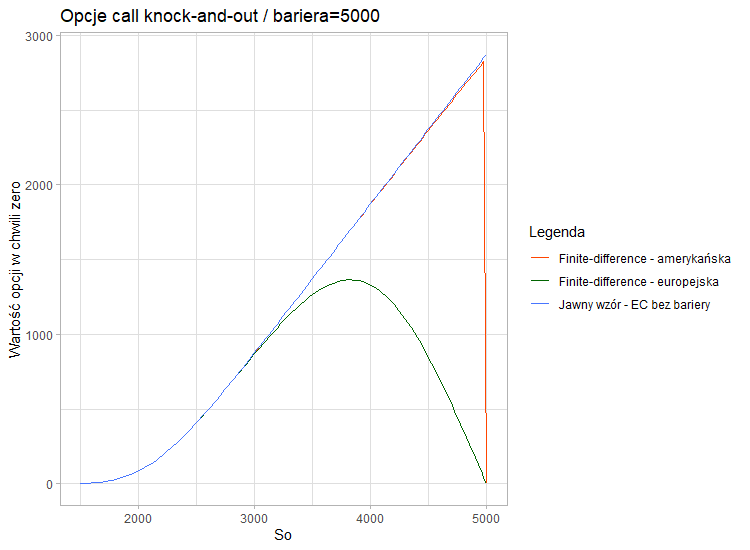
\includegraphics[width=0.8\textwidth,height=\textheight,keepaspectratio]{bariera5000.png}
    \caption{}
    \label{b5000}
\end{figure}

Rysunek \ref{b5000} pokazuje, co się dzieje jeśli odsuniemy barierę daleko od ceny wykonania. Zauważmy, że wycena europejskiej opcji barierowej dla wartości początkowych aktywa poniżej \(3000\) jest niemal identyczna jak wycena zwykłej opcji europejskiej.\\

\begin{figure}[H]
    \centering
    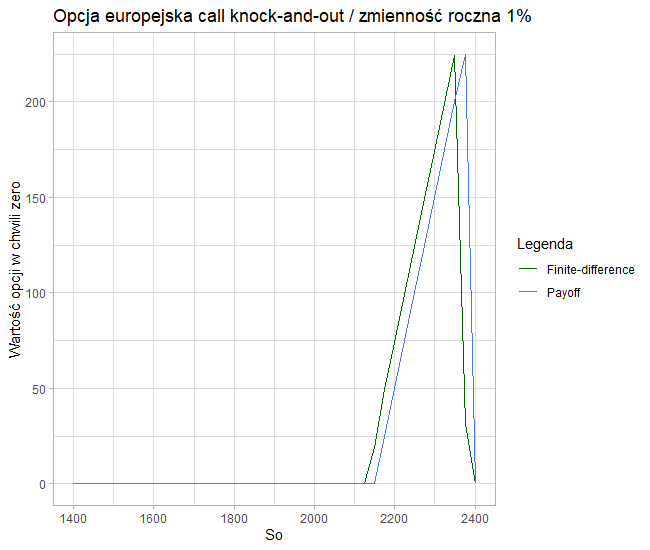
\includegraphics[width=0.8\textwidth,height=\textheight,keepaspectratio]{ec_sigma0.png}
    \caption{}
    \label{sigma0}
\end{figure}

Rysunek \ref{sigma0} ma za to obrazować, co się dzieje, gdy zmienność roczna zbliża się do zera. Można o tym myśleć w ten sposób, że sytuacja, w której mamy małą zmienność roczną jest analogiczna do sytuacji, w której zmienność jest większa, ale za to znajdujemy się blisko momentu wykonania, tzn. jest mało czasu na to aby cena aktywa znacznie się zmieniła. Z tego powodu wycena opcji jest bardzo zbliżona do payoffu.\\

Nasze intuicje oraz wyceny innymi metodami zgadzają się z otrzymanymi wynikami dla finite-difference, zatem możemy przypuszczać, że nasza implementacja jest poprawna.\\ 


Duża dokładność wyników, szybkie działanie oraz łatwość w dostosowaniu algorytmu do sytuacji (np. dywidendy, niepewna zmienność), czyni go dobrym narzędziem do wyceny instrumentów finansowych. Warto też dodać, że algorytm zwraca całą siatkę wyceny.


\end{document}
